\graphicspath{{system_id/fig/}, {system_id/plots}}

\chapter{System identification}
\label{chap:system_id}

    \paragraph
    System identification is the process of creating a mathematical model of a dynamical system 
    by using input and output measurements of that system.
    In this work a mathematical model of the multirotor and suspended payload system is required for swing damping control.
    The two major approaches to system identification are:
    \begin{enumerate}
        \item A priori mathematical modelling with parameter estimation
        \item Data-driven system identification
    \end{enumerate}

    \paragraph
    This chapter will discuss these approaches and describe the differences between them.
    For each approach, specific estimation techniques 
    will be applied to simulation data of the multirotor and payload system.
    The results of these techniques will then be discussed.

    \section{White-box and black-box techniques}

    \paragraph
    Models determined from data-driven system identification methods are generally called black-box models.
    The user is only concerned with the inputs and output of the model
    and does not determine mathematical relationships from theoretical deductions.
    In contrast, white-box models are determined from a priori modelling.
    The user understands the physics of white-box models 
    because the dynamics are manually programmed into the model by the user.

    \subsection{White-box techniques}

        \paragraph 
        The underlying physics of a white-box model is understood by the user because    
        it is determined from first principles.
        This is done by modelling physical processes with techniques like Lagrangian mechanics or Newton equations.
        For system identification techniques that use these models, 
        the mathematical relations between system parameters are predefined in the modelling phase.
        The system identification process is therefore reduced to parameter estimation 
        which determines values for the parameters used in die model.

        \paragraph 
        This approach is used by \cite{Erasmus2020} and \cite{Slabber2020} for swing damping control of a mulitrotor with an unknown suspended payload.
        The system was modelled as two rigid bodies connected by a link and the following assumptions were made regarding the suspended payload:
        \begin{itemize}
            \item The payload is a point mass.
            \item The link is massless.
            \item The link is rigid.
            \item The link is attached to the \gls{CoM} of the mulitrotor.
        \end{itemize}
        The only unknown parameters in the mulitrotor and payload model is the payload mass and the link length.
        These parameters are first estimated and then inserted into the predefined, linearised model.
        This model is used by a \gls{LQR} controller to damp swing angles while also controlling the vehicle.

        \paragraph 
        The approach works well for systems with predictable dynamics, but is not very adaptable to systems with slightly different dynamics.
        The payload considered by \cite{Erasmus2020} and \cite{Slabber2020} is limited to a small rigid mass suspended from the mulitrotor by a non-stretching cable. 
        In this configuration it was shown that a \gls{LQR} controller successfully controls a mulitrotor while minimising payload swing angles.
        However, if a payload or cable is used that violates one of the modelling assumptions, the predefined model no longer accurately represent the system.
        Many payloads which are considered for practical drone deliveries do not conform to these assumptions.
        Since the controller is dependent on this model, the mismatch between the model and actual dynamics may result in undesirable controller behaviour.

    \subsection{Black-box techniques}

        \paragraph
        Data-driven system identification methods produce black-box models.
        These models do not require predefined mathematical relations between system parameters.
        % The user only considers what goes into, and comes out of, the black-box.
        % Something imagery about why it is called black box
        No prior knowledge of the physics of the system are considered and no modelling assumptions are made.
        Black-box techniques determine the mathematical relationship between inputs and outputs of a system using information from measurement data only.

        \paragraph
        Dynamical models can be categorised as either non-linear or linear models.
        Non-linear models are often more accurate than linear models because complex, real-world dynamics are better approximated by non-linear systems.
        The dynamics of a mulitrotor and suspended payload are also non-linear.
        % Examples of black box models with mulitrotors and payloads in literature ???

        \paragraph
        However, non-linear models are inherently more complex than linear models. 
        Controllers based on non-linear models are usually more computationally complex than those with linear models.
        The control architectures used for mulitrotors in practical applications are mostly implemented on onboard hardware.
        Therefore there is value in low-complexity, linear models because these may be simple enough to execute on low cost hardware.
        % trade-off between accuracy and complexity.??
        Non-linear models may require control implementations that are too computationally expensive and may not be practically realisable on the available hardware on a mulitrotor.
        
        \paragraph
        \gls{DMDc} and \gls{HAVOK} are the two data-driven system identification methods investigated in this work. 
        These are linear regression techniques that produce linear models to approximate non-linear dynamics.
        Non-linear data-driven techniques like Neural Networks and SINDy \cite{Brunton2016a} may produce models that are more accurate than linear techniques, 
        but at the cost of greater computational complexity.
        % \murray{Name more techniques ??}
        \gls{DMDc} and \gls{HAVOK} are less computationally complex and their models are suitable for linear \gls{MPC}, which is significantly faster than non-linear \gls{MPC}.
        This is desirable for a practical mulitrotor implementation, where onboard computational power is limited.
        These techniques and their implementations are explained in the sections below.
        
        % \paragraph
        % Each technique is considered for use in a velocity controller in the North direction

        % 
    \section{Plant considered for system identification} \label{sec:plant_considered}
 
    % \paragraph
    % As discussed in \ref{sec:linear_model}, the payload is attached near the \gls{CoM} of the vehicle 
    % and has a minimal effect on the attitude dynamics.
    % The swing damping controllers are therefore applied in the translational velocity loop
    % and the original attitude controls are used for inner loop controllers.
    % Therefore the attitude state variables of the multirotor are excluded from the system identification model.

    % The model identified by \gls{DMDc} or \gls{HAVOKc} will be used to design a longitudinal velocity controller.
    % As shown in \ref{fig:system_id_plant}, the plant considered for system identification includes the dynamics of the inner loop, attitude controllers.
    % The swing damping controllers which will utilise the identified model act only in the translational velocity loop.
    % Because of the large time-scale separation between the inner and outer loop controllers, 
    % the attitude states have a negligible effect on the plant dynamics seen by the velocity controller.
    % As discussed in Section~\ref{sec:linear_model}, the payload minimally effects the multirotor attitude because it is attached near the \gls{CoM} of the vehicle.
    % Therefore the attitude states are excluded from the system identification model.

    \paragraph
    A specific subsystem of the multirotor-payload system will be considered for system identification.
    The proposed controllers in Chapter~\ref{chap:control} will be applied for North velocity control, therefore the longitudinal dynamics will be considered in this section.
    The input vector of the plant model is given by,
    \begin{equation}
        \bm{u} = \begin{bmatrix}
            A_{N_{sp}}
        \end{bmatrix} ,
    \end{equation}
    where $A_{N_{sp}}$ is the North acceleration setpoint in the inertial frame.
    $A_{N_{sp}}$ is used by the attitude controllers which will be explained in Section~\ref{sec:cascaded_pid}.
    The state vector of the considered plant is,
    \begin{equation}
        \bm{x} = \begin{bmatrix}
            V_N & \theta & \dot{\theta}
        \end{bmatrix}^T ,
    \end{equation}
    where $\theta$ and $\dot{\theta}$ are the payload angle and angular rate about the inertial East axis,
    and $V_N$ is the North velocity of the multirotor in the inertial frame. 
    A schematic of this \gls{2D} plant is shown in Figure~\ref{fig:floating_pend}, where $m_Q$ is the multirotor mass, $m_p$ is the payload mass, and $l$ is the cable length.

    \begin{figure}[htb]
        \centering
        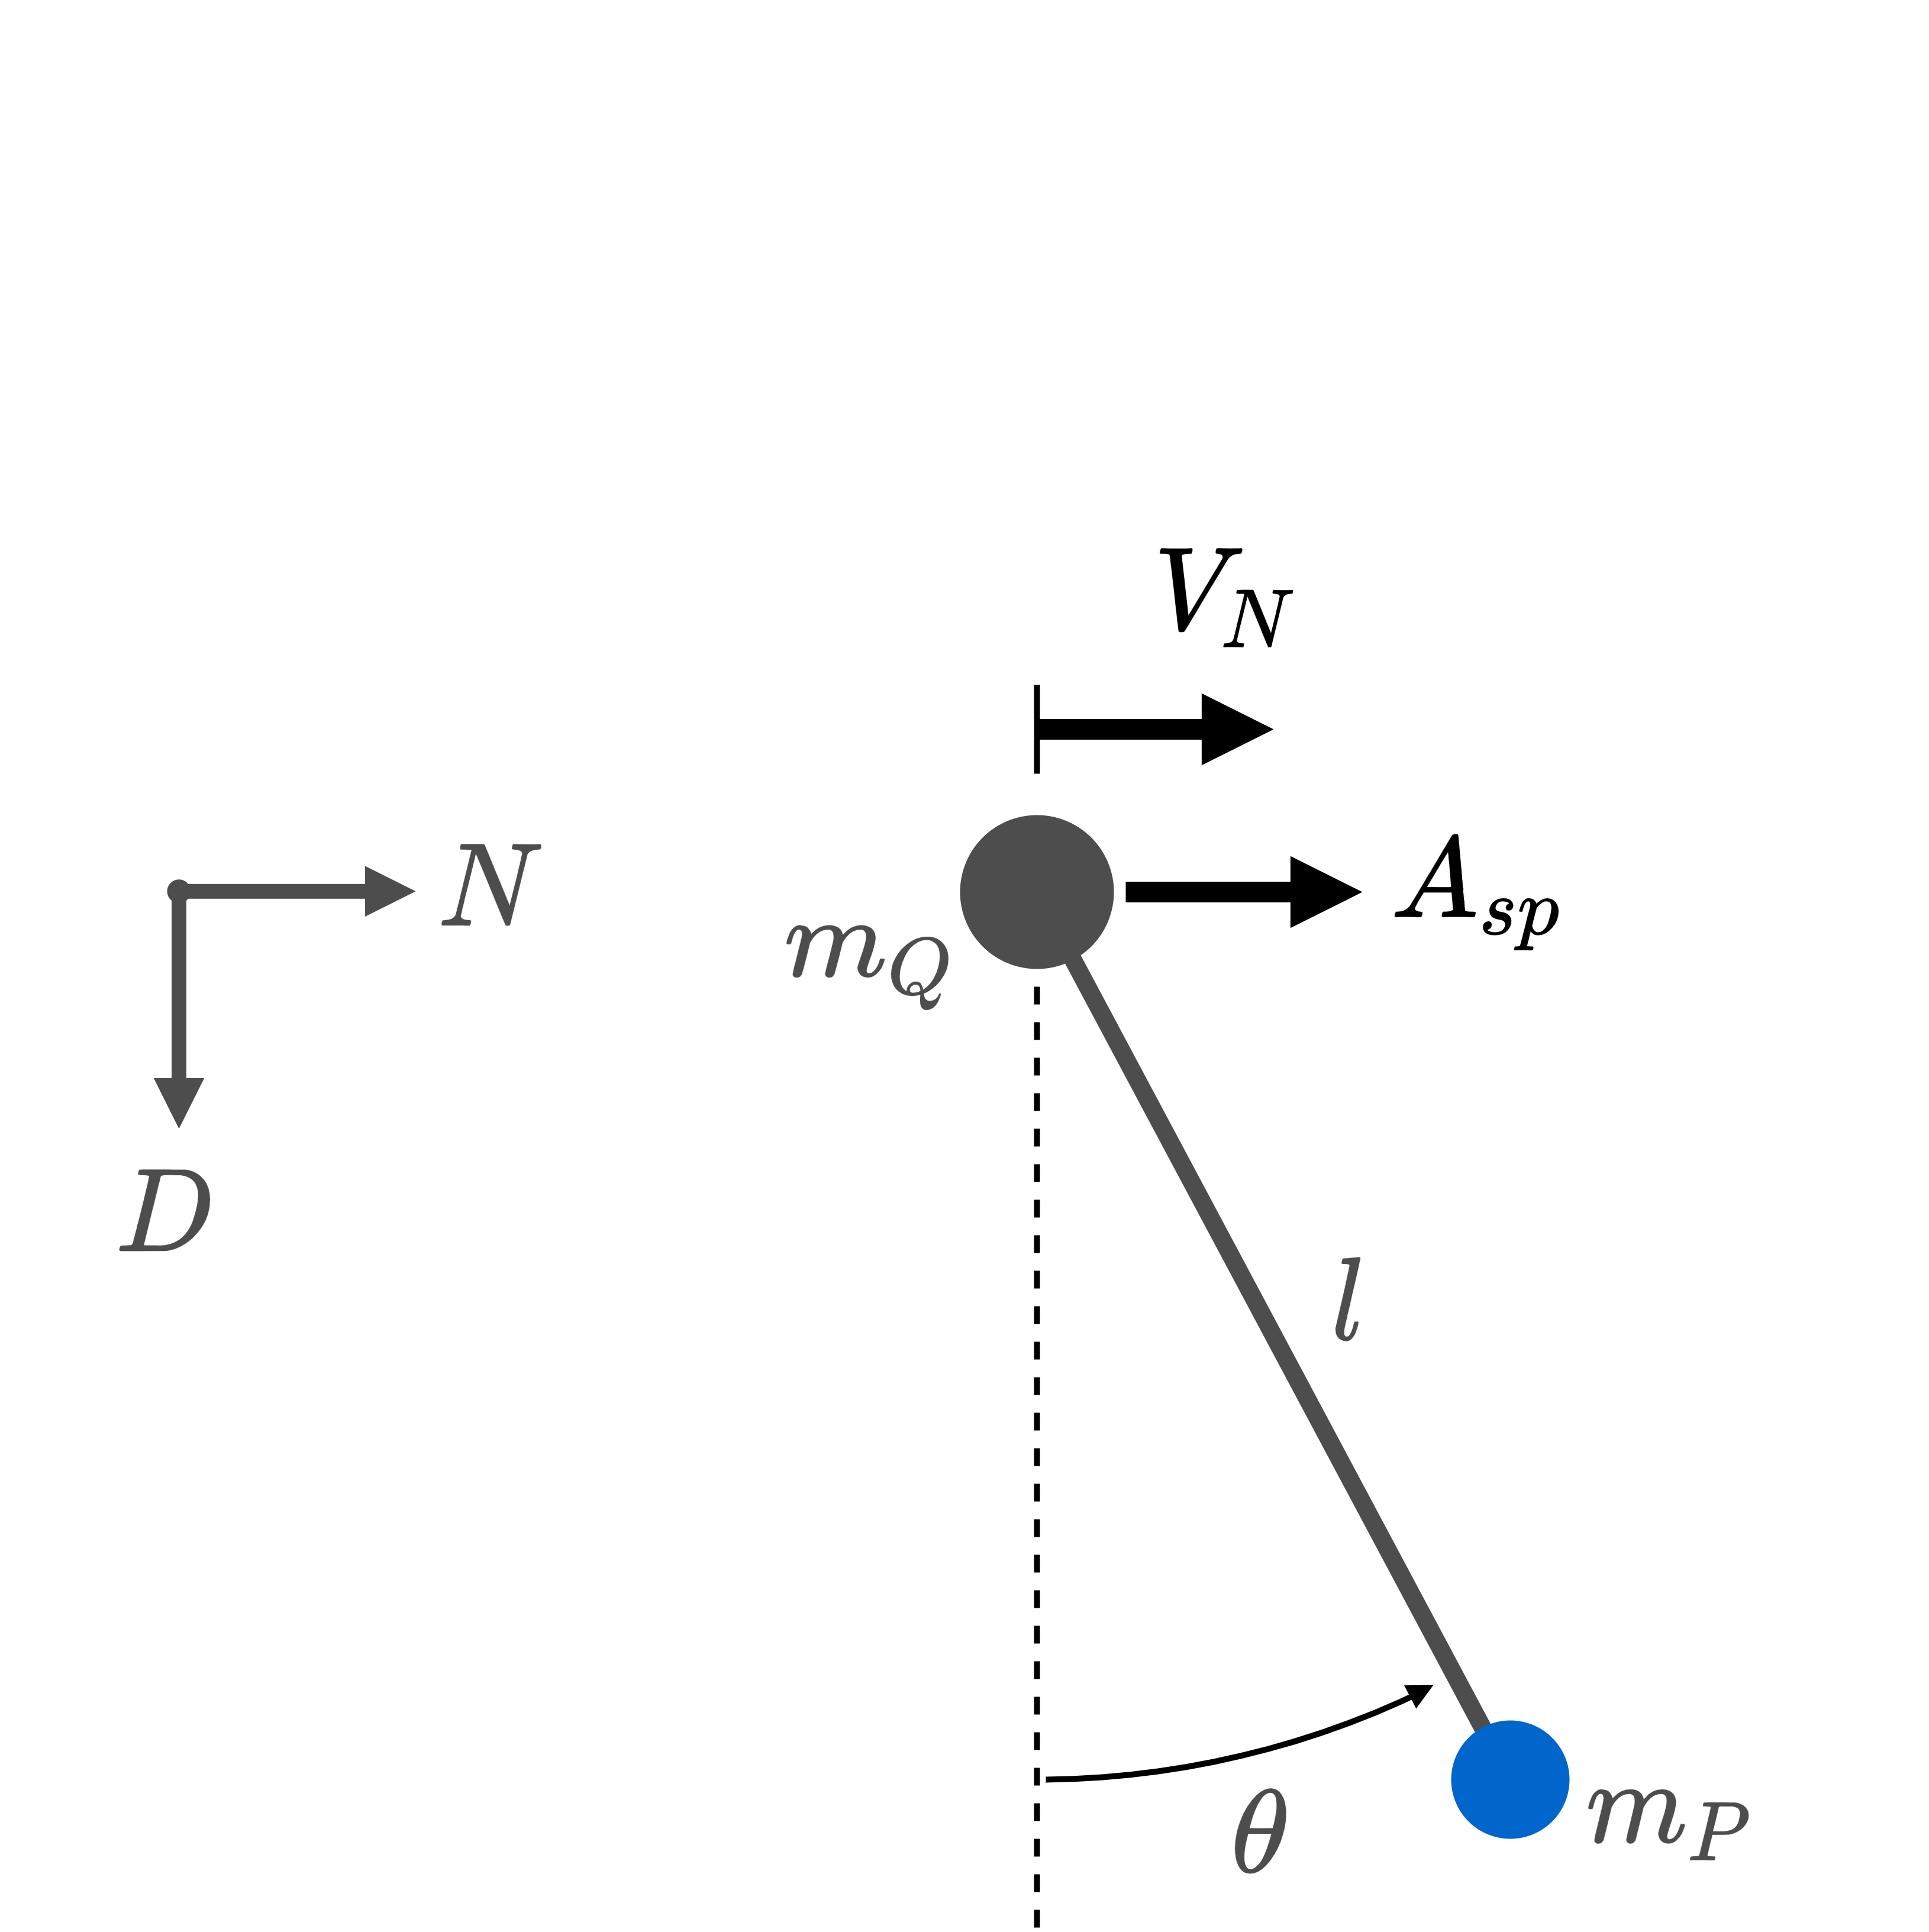
\includegraphics[width=0.45\linewidth]{floating_pend.png}            
        \caption{Schematic of a floating pendulum model considered for a North velocity controller}
        \label{fig:floating_pend}
    \end{figure}

    % Also note that the inner loop controllers handle the attitude dynamics of the multirotor.
    % During simulations of pure longitudinal velocity setpoints, 
    % it was observed that the multirotor experiences negligible altitude changes due the swinging payload.
    % This is due to the speed of the altitude controllers and the weak coupling between the payload angle and the altitude dynamics, 
    % discussed in Chapter~\ref{chap:modelling}.
    % The plant seen by the system identification process therefore mimics the common pendulum-on-a-cart model.
    
    % The differential equations that describe the motion of this system 
    % were derived with Lagrangian mechanics in Chapter~\ref{chap:modelling}.

    % From this derivation it is clear that the angular velocity of the payload, $\dot{\theta}$, is required to described the system dynamics.
    % However, $\dot{\theta}$ is not measured directly on the considered practical multirotor setup.
    % Instead, the payload angle, $\theta$, is measured by a potentiometer attached to a \gls{ADC} on Honeybee as described in Chapter \ref{chap:exp_design}.
    % As expected, this measurement is extremely noisy.
    % \murray{Maybe insert figure to show noise}
    % % Figure \ref{} shows the angle measurement during a practical experiment of the payload while Honeybee is held stationary
    % Numerical differentiation is applied to the noisy $\theta$ signal which results in a very inaccurate estimation of $\dot{\theta}$.
    % Therefore it is desirable to rather use $\theta$ in the system identification process. 
    
    \paragraph
    In subsequent sections, simulations of the full, non-linear multirotor-payload system will be performed
    and different methods will be applied to determine system identification models of this plant.

    \section{Parameter estimation}
\subsection{Predetermined linear model}
    The motivation for paramater estimation is to determine unknown parameter values required by the predetermined model.
    This model was derived a prioiri in Section~\ref{sec:linear_model}.
    
\subsection{Payload mass estimation}
    RLS

\subsection{Cable length estimation}
    The cable length is estimated from the measurement of natural frequency of the swinging payload.
    As described by
    \cite{bisgaard},
    the natural frequency is given by:
    \begin{equation} \label{eq:nat_freq}
        \omega_n = \sqrt{ \frac{g}{l} \cdot \frac{m_q + m_p}{m_q}}
    \end{equation}
    The natural frequency is measured by performing a FFT on the payload swing angle response after a position step by the quadrotor.
    The dominant frequency identified by the FFT during free swing is the natural frequency of the payload.
    
    \ref{fig:pos_step_angle}
    shows the payload swing angle after the system is stimulated by a position step setpoint.
    As shown in 
    \ref{fig:pos_step_angle}
    the first few seconds of the step response are not used in the FFT.
    This is to minimise the effect of the quadrotor controllers on the swing angle frequency 
    by excluding the transient response in the FFT.

    \ref{fig:fft} 
    shows the resulting amplitude spectrum of the payload swing angle response.
    The dominant frequency is clearly identified as ??.
    Since $m_q$ and $g$ is known, and $m_p$ and $\omega_n$ has been estimated, $l$ can now be determined from
    \ref{eq:nat_freq}.
    In this case the estimated length is ??, compared to the actual length of ??.
    
    Frequency resolution ??
    error for different lengths??


    \section{Dynamic mode decomposition with control}
\label{sec:dmdc}
    
    \paragraph        
    \gls{DMD} is a regression technique that can be used to approximate a non-linear dynamical system with a linear model \cite{Tu2014}.
    It uses temporal measurements of system outputs to reconstruct system dynamics without prior modelling assumptions.
    \gls{DMDc} is an adaptation of \gls{DMD} that also accounts for control inputs \cite{Proctor2016c}.
    This section provides an overview of the specific implementation of \gls{DMDc} used in this work.        
    Note that this implementation is an adaptation of \gls{DMDc}, and includes time-delay-embedding of multiple variables. 
    Enriching a \gls{DMD} model with time-delay-embedding is a known technique and is also seen in other \gls{DMD} adaptations \cite{Korda2018b, Arbabi2018}.

    \paragraph
    \gls{DMD} produces a linear, discrete state-space model of system dynamics.
    Discrete measurements, $\bm{x}_k$, of the continuous time variable, $\bm{x}(t)$, are used, 
    where $\bm{x}_k = \bm{x}(k T_s)$, and $T_s$ is the sampling time of the model.    
    Delay-coordinates (i.e. $\bm{x}_{k-1}, \bm{x}_{k-2}$, etc.) are also included in the state-space model to
    account for input delay and state delay in the system.
    Input delay refers to the time delay involved with transporting a control signal to a system, 
    whereas state delay refers to time-separated interactions between system variables \cite{Chen1999}.
    Hence, we define a state delay vector as:
    \begin{equation} \label{eq:delay_vector}
        \bm{d}_{k} = 
        \begin{bmatrix}
            \bm{x}_{k-1} & \bm{x}_{k-2} & \cdots & \bm{x}_{k-q+1}
        \end{bmatrix}^T ,
    \end{equation}
    where 
    $q$ is the number of delay-coordinates 
    (including the current time-step) used in the model, and $\bm{d}_k \in \R^{(n_x)(q-1)}$.
    
    \paragraph
    The discrete state-space model is therefore defined as:
    \begin{equation} \label{eq:dmd_state_space}
        \bm{x}_{k+1} = \bm{A}_{dmd} \bm{x}_k + \bm{A}_d \bm{d}_k + \bm{B}_d \bm{u}_k ,
    \end{equation}
    where
    \( \bm{A}_{dmd} \in \R^{n_x \times n_x} \) is the system matrix, 
    \( \bm{A}_d \in \R^{(q-1) \cdot n_x ~ \times ~ (q-1) \cdot n_x} \) is the state delay system matrix and 
    \( \bm{B}_d \in \R^{n_x \times n_u} \) is the input matrix.
    
    \paragraph
    The training data consists of full-state measurements, $\bm{x}_k$, and corresponding inputs, $\bm{u}_k$, 
    taken at regular intervals of $\Delta t = T_s$, during a simulated flight with Cascaded \gls{PID} control.
    In a practical flight, these time-series measurements need to be saved in memory because it is processed as a single batch by \gls{DMD}.
    Note that \gls{DMD} can be applied in a recursive manner as described in \cite{Noack2016}.
    However, this implementation is not considered because an \gls{OBC} with significant memory size can be used.
    
    \paragraph
    The training data is collected into the following matrices:
    \begin{align} \label{eq:dmd_matrices}
        \bm{X^\prime} = & \phantom{.} \left [
            \begin{array}{*{5}{@{}M{\mycolwd}@{}}}
                    \bm{x}_{q+1} & \bm{x}_{q+2} & \bm{x}_{q+3} & \cdots & \bm{x}_{w+q}
            \end{array}
        \right ] , \nonumber \\
        %
        \bm{X} \phantom{''} = & \phantom{.} \left [
            \begin{array}{*{5}{@{}M{\mycolwd}@{}}}
                \bm{x}_{q} & \bm{x}_{q+1} & \bm{x}_{q+2} & \cdots & \bm{x}_{w+q-1}                      
            \end{array}
        \right ] , \nonumber \\
        % 
        \bm{X}_d \phantom{'} = & \phantom{'} \left [
            \begin{array}{*{5}{@{}M{\mycolwd}@{}}}
                \bm{x}_{q-1} & \bm{x}_{q+0} & \bm{x}_{q+1} & \cdots & \bm{x}_{w+q-2} \\
                \vdots   & \vdots   & \vdots   & \ddots & \vdots \\
                \bm{x}_2 & \bm{x}_3 & \bm{x}_4 & \cdots & \bm{x}_{w+1} \\
                \bm{x}_1 & \bm{x}_2 & \bm{x}_3 & \cdots & \bm{x}_{w} \\                       
            \end{array}
        \right ] , \nonumber \\
        % 
        \bm{\Upsilon} \phantom{'} = & \phantom{.} \left [
            \begin{array}{*{5}{@{}M{\mycolwd}@{}}}
                    \bm{u}_{q} & \bm{u}_{q+1} & \bm{u}_{q+2} & \cdots & \bm{u}_{w+q-1}
            \end{array}
        \right ] ,
    \end{align}
    where $w$ is the number of columns in the matrices, 
    $\bm{X^\prime}$ is the matrix $\bm{X}$ shifted forward by one time-step, 
    $\bm{X}_d$ is the matrix with delay states, 
    and $\bm{\Upsilon}$ is the matrix of inputs.
    Equation~\ref{eq:dmd_state_space} can be combined with the matrices in Equation~\ref{eq:dmd_matrices} to produce:
    \begin{equation}
        \bm{X^\prime} = \bm{A}_{dmd} \bm{X} + \bm{A}_d \bm{X}_d + \bm{B}_d \bm{\Upsilon} .
    \end{equation}
    Note that the primary objective of \gls{DMDc} is to determine the best fit model matrices, $\bm{A}_{dmd}$, $\bm{A}_d$ and $\bm{B}_d$, 
    given the data in $\bm{X^\prime}$, $\bm{X}$, $\bm{X}_d$, and $\bm{\Upsilon}$ \cite{Proctor2016c}.
    In order to group the unknowns into a single matrix, Equation~\ref{eq:dmd_state_space} is manipulated into the form,
    \begin{equation} \label{eq:G_Omega}
        \bm{X^\prime} =   
        \begin{bmatrix} 
            \bm{A}_{dmd} & \bm{A}_d & \bm{B}_d 
        \end{bmatrix}
        \begin{bmatrix} 
            \bm{X} \\ \bm{X}_d \\ \bm{\Upsilon} 
        \end{bmatrix} 
        = \bm{G \Omega} ,
    \end{equation} 
    where $\bm{\Omega}$ contains the state and control data, and $\bm{G}$ represents the system and input matrices.
    
    \paragraph
    A \gls{SVD} is performed on $\bm{\Omega}$ resulting in:
    \(
        \bm{\Omega} = \bm{U} \bm{\Sigma} \bm{V}^T
    \).
    Often, only the first $p$ columns of $\bm{U}$ and $\bm{V}$ are required for a good approximation of the dynamics \cite{Brunton2017a}.
    % Talk about Reduced Order Modelling??
    % \gls{POD} modes??
    In many cases, the truncated form results in better models than the exact form when noisy measurements are used.
    This is because the effect of measurement noise is mostly captured by the truncated columns of $\bm{U}$ and $\bm{V}$.
    By truncating these columns, the influence of noise in the regression problem is reduced. 
    % \murray{explain this better ??}
    Hence the \gls{SVD} is used in the truncated form: 
    \begin{equation} \label{eq:tilde_svd}
        \bm{\Omega} \approx \Tilde{\bm{U}} \Tilde{\bm{\Sigma}} \Tilde{\bm{V}}^T ,
    \end{equation}
    where $\phantom{.} \Tilde{ } \phantom{.}$ represents rank-$p$ truncation.
    For the $\bm{U}$ and $\bm{V}$ matrices, rank-$p$ truncation refers to keeping only the first $p$ number of columns and truncating the rest.
    Rank-$p$ truncation of the $\bm{S}$ matrix refers to keeping the first $p$ number of columns and rows and truncating the rest.
    % \murray{maybe insert colour pictures showing matrices ??}        

    \paragraph
    By combining Equation~\ref{eq:tilde_svd} with the over-constrained equality in Equation~\ref{eq:G_Omega}, 
    the least-squared solution, $\bm{G}$, can be found with:
    \begin{equation}
        \bm{G} \approx \bm{X^\prime} \Tilde{\bm{V}} \Tilde{\bm{\Sigma}}^{-1} \Tilde{\bm{U}} .
    \end{equation}
    By reversing Equation~\ref{eq:G_Omega}, $\bm{G}$ can now be decomposed into:
    \(
        \bm{G} = \begin{bmatrix} \bm{A}_{dmd} & \bm{A}_d & \bm{B}_d \end{bmatrix}
    \)
    according to the required dimensions of each matrix.
    Thereby, the state-space model approximated by \gls{DMDc} is complete.
    

    \section{Hankel alternative view of Koopman} 
\label{sec:havok}
    
    \paragraph
    HAVOK is a data-driven, regression technique that provides a connection 
    between DMD and Koopman operator theory \cite{Brunton2017a, Champion2019}. 
    We have adapted the standard HAVOK algorithm slightly to account for the effect of control and to extract a discrete, linear model that approximates the behaviour of a controlled dynamical system.
    In this section, a brief overview is provided for this implementation and adaptation of HAVOK.
    % 
    \paragraph
    A defining characteristic of HAVOK is that it uses multiple delay-coordinates (i.e. $\bm{x}_{k-1}, \bm{x}_{k-2}$, etc.) 
    in the system identification process.
    To fit this into the standard state-space format, an extended state vector is defined as:
    \begin{equation}
         \bm{a}_{k} = \begin{bmatrix} \bm{x}_{k-(q-1)} & \cdots & & \bm{x}_{k-1} & & \bm{x}_{k} \end{bmatrix}^T ,
    \end{equation}
    where $\bm{a}_k \in \R^{(n_y)(q)}$, and the subscript of $\bm{a}$ denotes the highest subscript of ${\bm{x}}$ in the vector.
    
    \paragraph
    The resulting discrete state-space model is therefore in the form,
    \begin{equation} \label{eq:havok_state_space}
        \bm{a}_{k+1} = \Tilde{\bm{A}} \bm{a}_k + \Tilde{\bm{B}} \bm{u}_k ,
    \end{equation}
    where \( \Tilde{\bm{A}} \in \R^{(q \cdot n_x) \times (q \cdot n_x)} \) is the system matrix, 
    and \( \Tilde{\bm{B}} \in \R^{(q \cdot n_x) \times n_u} \) is the input matrix. 
    Here, $\Tilde{\phantom{a}}$ is used to differentiate these matrices from $\bm{A}$ and $\bm{B}$ used in DMDc.
    % 
    \paragraph
    The original HAVOK algorithm, developed by \cite{Brunton2017}, constructs a Hankel matrix from output variables only. 
    In this work, the standard HAVOK algorithm has been adapted to incorporate the effect of control.
    An extended Hankel matrix, $\bm{\Pi}$, is created by appending a matrix of inputs to a Hankel matrix of measurements:
    \begin{equation} \label{eq:pi_hankel}
        \bm{\Pi} = \phantom{.} \left [
            \begin{array}{*{5}{@{}M{\mycolwd}@{}}}
                    \bm{a}_{q} & \bm{a}_{q+1} & \bm{a}_{q+2} & \cdots & \bm{a}_{w+q-1} \\
                    \bm{u}_{q} & \bm{u}_{q+1} & \bm{u}_{q+2} & \cdots & \bm{u}_{w+q-1}
            \end{array}
        \right ] ,
    \end{equation}
    where $w$ is the number of columns in $\bm{\Pi}$.
    A truncated SVD of this Hankel matrix results in following approximation:
    \begin{equation} \label{eq:havok_svd_tilde}
        \bm{\Pi} \approx \Tilde{\bm{U}} \Tilde{\bm{\Sigma}} \Tilde{\bm{V}}^T ,
    \end{equation}
    where $\Tilde{\phantom{a}}$ represents rank-$p$ truncation.
    It is important to note that the model extracted by HAVOK depends on the choice of hyperparameters ($p$ and $q$),
    and the number of training samples ($N_{train} = w + q -1$).
    
    \paragraph
    The columns of $\Tilde{\bm{V}}$ are the most significant principal components of the system dynamics \cite{Kamb2020}.
    This matrix, $\Tilde{\bm{V}}$, can be considered to contain a time-series of the pseudo-state, $\bm{v}$, such that
    \(
        \Tilde{\bm{V}}^T = \begin{bmatrix} 
            \bm{v}_q & \bm{v}_{q+1} & \cdots & \bm{v}_w 
        \end{bmatrix} ,
    \)
    characterises the evolution of the actual dynamics in an eigen-time-delay coordinate system \cite{Brunton2017}.
    % 
    Consider the following discrete, state-space formulation:
    \begin{equation} \label{eq:v_ss}
        \bm{v}_{k+1} = \bm{\Lambda} \bm{v}_k .
    \end{equation}
    HAVOK determines the best fit linear operator $\bm{\Lambda}$ that maps the pseudo-state $\bm{v}_k$ to $\bm{v}_{k+1}$.
    In order to setup an over-determined equality for (\ref{eq:v_ss}), $\Tilde{\bm{V}}^T$ is divided into two matrices:
    \begin{align} \label{eq:v1v2}
        \bm{V}_1 &= \left [
            \begin{array}{*{5}{@{}M{\mycolwd}@{}}} 
                \bm{v}_{q \phantom{-1}}     & \bm{v}_{q+1} & ... & \bm{v}_{w-1} \\
            \end{array} 
        \right ] , \nonumber \\ 
        \bm{V}_2 &= \left [
            \begin{array}{*{5}{@{}M{\mycolwd}@{}}} 
                \bm{v}_{q+1}     & \bm{v}_{q+2} & ... & \bm{v}_{w \phantom{-1}} \\
            \end{array} 
        \right ] ,
    \end{align} 
    where $\bm{V}_2$ is $\bm{V}_1$ advanced a single step forward in time.
    The matrices from Equation (\ref{eq:v1v2}) are now combined with Equation (\ref{eq:v_ss}) and the best fit $\bm{\Lambda}$ is determined with the Moore-Penrose pseudoinverse:
    \begin{equation} \label{eq:v_dmd}
        \bm{V}_2 = \bm{\Lambda} \bm{V}_1 \phantom{---} \Rightarrow \phantom{---} \bm{\Lambda} \approx \bm{V}_1 \bm{V}_1^{\dagger}
    \end{equation}
    % 
    It can be shown from Equation (\ref{eq:havok_svd_tilde}) that Equation (\ref{eq:v_ss}) is transformed from the eigen-time-delay coordinate system to the original coordinate system as the following:
    \begin{equation} \label{eq:v_ss_a} 
        \begin{bmatrix}
            \bm{a}_{k+1}  \\  \bm{u}_{k+1} 
        \end{bmatrix}
    \phantom{.} = \phantom{.} (\Tilde{\bm{U}} \Tilde{\bm{\Sigma}}) \bm{\Lambda} (\Tilde{\bm{U}}  \Tilde{\bm{\Sigma}})^{\dagger} \phantom{.}
        \begin{bmatrix}
            \bm{a}_{k}  \\  \bm{u}_{k} 
        \end{bmatrix} .
    \end{equation}    
    % 
    % This form is used to extract $\Tilde{\bm{A}}$ and $\Tilde{\bm{B}}$ from the matrix,
    % \( 
    %     (\Tilde{\bm{U}} \Tilde{\bm{\Sigma}}) \bm{\Lambda} (\Tilde{\bm{U}}  \Tilde{\bm{\Sigma}})^{\dagger}
    % \), in the following way:
    % \begin{equation} \label{matrix_decomp}
    %     \begin{bmatrix}
    %         \bm{a}_{k+1}  \\  \bm{u}_{k+1} 
    %     \end{bmatrix}
    %     \phantom{.} = \phantom{.} 
    %     \begin{bmatrix}
    %         \Tilde{\bm{A}} \phantom{.....} \Tilde{\bm{B}} \\
    %         \textit{(discarded)}
    %     \end{bmatrix}
    %     \phantom{.}
    %     \begin{bmatrix}
    %         \bm{a}_{k}  \\  \bm{u}_{k} 
    %     \end{bmatrix}.
    % \end{equation}    
    
    \paragraph
    $\Tilde{\bm{A}}$ and $\Tilde{\bm{B}}$ can now be extracted from the matrix,
    \( 
        (\Tilde{\bm{U}} \Tilde{\bm{\Sigma}}) \bm{\Lambda} (\Tilde{\bm{U}}  \Tilde{\bm{\Sigma}})^{\dagger}
    \).
    This extraction is illustrated in Figure~\ref{fig:havok_decomposition}, 
    where different blocks represent different groups of matrix entries.
    \begin{figure}[h]
        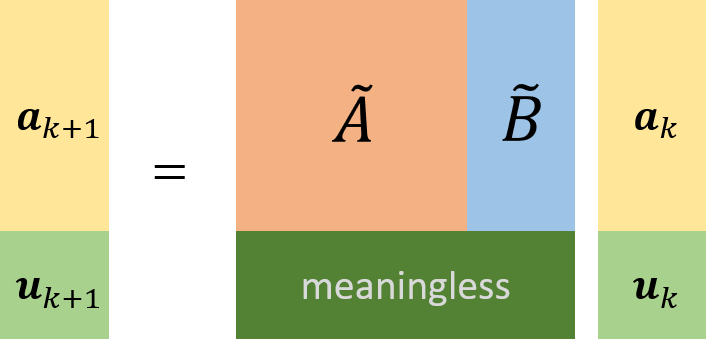
\includegraphics[scale = 0.55]{havok_decomposition.png}
        \centering
        \caption{Illustration of the extraction of $\Tilde{\bm{A}}$ and $\Tilde{\bm{B}}$ from (\ref{eq:v_ss_a})}
        \label{fig:havok_decomposition}
    \end{figure}
    
    \paragraph
    Note that the matrix entries in Figure~\ref{fig:havok_decomposition} that map $\bm{u}_k$ to $\bm{u}_{k+1}$ 
    are meaningless for state predictions and are discarded.
    Also note that the state vector, $\bm{a}_k$, includes delay-coordinates, therefore some matrix entries are independent of the dynamics.
    This is illustrated in Figure~\ref{fig:havok_force_entries} for an example model with $q = 4$.
    For example, the mapping of $\bm{x}_k$ in the state vector to $\bm{x}_k$ in the predicted state vector
    corresponds to a entry of 1 in the $\Tilde{\bm{A}}$ matrix.
    This is fixed by the model format and is not a function of the system dynamics.
    Due to the least-squares fitting and the coordinate transformation of the algorithm, 
    HAVOK does not produce these exact values in $\Tilde{\bm{A}}$ and $\Tilde{\bm{B}}$. 
    By forcing each of these matrix entries to 1 or 0, the state-prediction performance of the model is improved.
        
    \begin{figure}[h]
        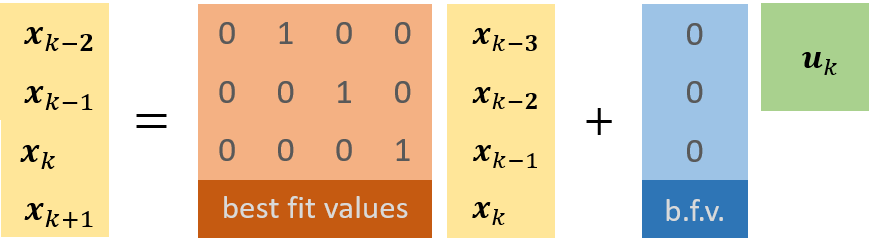
\includegraphics[scale = 0.75]{havok_force_entries.png}
        \centering
        \caption{Illustration of }
        \label{fig:havok_force_entries}
    \end{figure}

    \paragraph
    Finally, the improved $\Tilde{\bm{A}}$ and $\Tilde{\bm{B}}$ are inserted into (\ref{eq:havok_state_space}) to render the HAVOK model.
    





    \section{Implementation and results}

    In order to test the system identification techniques,
    numerous simulations were performed to investigate their performance 
    with different system configurations.
    Firstly, the influence of design parameters on the algorithm performance are explored.
    These parameters include hyperparameters, the length of training data and the algorithm sample time.
    The effect of conditions that are not determined by algorithm design are also explored, 
    like measurement noise, and the physical properties of the payload.
    Finally, the white-box and black-box techniques are tested on a dynamic payload 
    which does not satisfy the assumptions of a simple pendulum.

    \subsection{Methodology}

        \paragraph{}
        A SITL implementation of PX4 \cite{Meier2015} using the Gazebo simulator \cite{Koenig2004} is used to generate data
        for system identification.
        Testing these techniques with simulation data allow us to investigate a much larger range system configurations 
        than possible with practical flights.
        The simulation model used in Gazebo was verified in Chapter~\ref{chap:modelling}.
        Using PX4 in SITL also ensures that the controller dynamics in simulation 
        is as close as possible to practical flights since the same flight stack is used in both cases.
        Gazebo also applies realistic measurement noise to the signals received by PX4, 
        which applies an EKF for state estimation.
        Therefore the the data seen by the system identification techniques 
        will also include the filtering effect of the EKF as it would in practical flights.

        \paragraph{}
        The procedure used to evaluate the black-box techniques is as follows:
        \begin{enumerate}
            \item Takeoff and hover with the qaudrotor
            \item Start logging input and output data
            \item Command a series of velocity step setpoints with random step sizes and time intervals
            \item Stop logging data
            \item Split data into separate training and testing periods
            \item Build a model from the training data
            \item Calculate a error metric for the model from the testing data
        \end{enumerate}

        \paragraph{}
        The default PID velocity controller from PX4 is used during these simulation.
        The implemented controller gains are documented in Appendix~\ref{appen:pid_gains}.
        A ROS node is used to read and log the payload angle measurement from Gazebo and a different
        ROS node is used to send the velocity setpoints to PX4 
        through the MAVLink protocol with the ROS package, 'mavros'.

        \paragraph{}
        A algorithm schedules the series of velocity step commands 
        by assigning random step values and time-intervals within a specified range.
        Theses values are selected from a uniform distribution 
        within the ranges specified in Table~\ref{tbl:input_ranges}
        The maximum velocity step is determined in simulation by iteratively increasing the maximum velocity step 
        to a safe value where the quadrotor remains in stable flight
        and the payload angles do not swing out of control.
        The time interval range is set iteratively to ensure 
        that the generated data includes both transient and steady-state dynamics.
 
        \begin{table}[!h]
            \renewcommand{\arraystretch}{1.1}
            \centering
            \caption{Input data ranges.}
            \begin{tabularx}{0.65\linewidth}{@{}lCCr@{}}
                \toprule
                         & Velocity step [\SI{}{\metre/\second}]  & Step time interval [\SI{}{\second}]\\
                \midrule
                Minimum  & 0                                    & 10\\
                Maximum  & 3                                    & 25\\
                \bottomrule
            \end{tabularx}
            \label{tbl:input_ranges}
        \end{table}
        
        \begin{figure}[!htb]
    \centering
    \begin{tikzpicture}
        \begin{axis}[            
            xlabel = Time,
            ylabel = North velocity,
            x unit = \si{\second},
            y unit = \si{\radian},
            xmin = 0,   xmax = 200,
            ymin = -2.5,  ymax = 2.5,
            grid = major,
            legend cell align = left,
            legend pos = north east,
            grid style = dashed,
            legend style = {font = \scriptsize},
            label style = {font = \scriptsize},
            tick label style = {font = \scriptsize},
            width = 0.95\columnwidth,
            height = 0.5\columnwidth,
            % initialize Dark2
            cycle list/Dark2,
            % combine it with 'mark list*':
            cycle multiindex* list = {
                Dark2\nextlist
            }
        ]
        
        \addplot+[mark = none, style = solid, ultra thick] 
        table[x = time, y = vel_sp, col sep = comma] 
        {system_id/csv/training_data_SITL_x_vel_noise_l1_m0-2.csv.csv};
        \addlegendentry{$V_{N,sp}$}
        
        \addplot+[mark = none, style = solid, ultra thick] 
        table[x = time, y = vel, col sep = comma] 
        {system_id/csv/training_data_SITL_x_vel_noise_l1_m0-2.csv.csv};
        \addlegendentry{$V_N$}

        \end{axis}
    \end{tikzpicture} 
    
    \caption{Example of training data with random velocity step inputs
        ($m_p =$~\SI{0.2}{\kilo\gram}, $l =$~\SI{1}{\meter})}
    \label{fig:training_data}
\end{figure}


        \paragraph{}
        Figure~\ref{fig:training_data} 
        shows an example of random velocity steps and the resulting velocity response used as training data.
        Using random velocity steps and time intervals prevents the system identification methods 
        from overfitting to a specific set of control conditions.
        The method should rather determine a generalised model 
        that works over a range of possible control conditions.

        \paragraph{}
        The data logged from simulation is then divided into testing and training data.
        The training data is used by the system identification algorithms to generate a regression model 
        and the model is then used to determine a prediction error metric over the unseen testing data.
        It is common practice in model evaluations 
        to use separate sets of data for training and testing.
        This ensures that good predictions scores do not result from models that overfit to the training data. 
        
        \paragraph{}
        The testing data spans a fixed length of time and taken from the start of the simulation period.
        The training data is then allocated from the remainder of the data.
        The same testing data is used to calculate error metrics for different models with different configurations
        to ensure that the metric for each model is comparable. 
        This error metric calculated from the testing data is used to evaluate and rank the performances of different models.       

        % \paragraph{Why velocity steps?}
        % As discussed before, the purpose of identifying a data-driven model of the plant dynamics 
        % is to use it in a MPC controller in the velocity loop, 
        % therefore velocity inputs are used in the system identification process.
        % It is a common technique to use a step responses for system identification \cite{Chen2011} because it exposes a 
        % large range of frequency data in the system dynamics.
        % In other data-driven techniques like Neural-Nets, it may be helpful to use a larger variety of input types.
        % The input schedule may be generated by randomly switching between step, ramp and exponetional inputs 
        % to further gaurd againts overfitting \cite{Kotze2021}.
        % However, for the 
        % In practice it is more common to command position step setpoints since a quadrotor delivers

    \subsection{Error metric}

        \paragraph{}        
        It is common practice is to select a model for a MPC based on k-step-ahead prediction errors \cite{Zhao2014}.
        This is because the model is used to make k-step-ahead predictions during control optimisation.
        When model error is dominated by variance error (caused by disturbances), 
        it may be better to use one-step-prediction error \cite{Zhao2014}.
        However for the quadrotor and payload case it is assumed that variance error 
        (caused by under modelling) dominates the model error.

        \paragraph{}
        Different metrics are used in literature to quantify prediction accuracy for different applications.
        Very common, scale-dependant error metrics are MSE and MAE.
        These metrics are dependant on the unit and scale of a variable, 
        hence they cannot be used to compare predictions of different variables.
        MSE ($l_2$~norm of error values) penalises larger errors more than smaller errors, 
        whereas MAE ($l_1$~norm) penalises errors equally.
        For our use case the $l_1$~norm provides a more intuitive metric than the $l_2$~norm
        because it has the same unit as the prediction variable
        and there is no motivation to penalise larger errors more than smaller errors for our use case.

        \paragraph{}
        MAE is calculated as:
        % \begin{equation}
        %     \bm{MAE} = \frac{1}{N_{run}} \cdot \sum_{k = 1}^{N_{run}} \left\lvert \bm{\hat{x_k}} - \bm{x_k} \right\rvert ,
        % \end{equation}
        \begin{equation}
            \bm{MAE} = mean \left( \phantom{.} \left\lvert \bm{\hat{x_k}} - \bm{x_k} \right\rvert \phantom{.} \right),
        \end{equation}
        where 
        % $N_{run}$ is the number of samples used in the prediction run,
        $\bm{x_k}$ is the actual state vector at time-step $k$, 
        $\bm{\hat{x_k}}$ is the state prediction, 
        and 
        $\bm{MAE}$ is a vector with the MAE of each state.
        
        \paragraph{}
        Popular, scale-free error metrics, like MAPE, MRAE and MASE, are also based on the $l_1$~norm,
        but are independent of the scale and units of a variable \cite{Hyndman2006}.
        These metrics could therefore be used to compare predictions of different variables.
        However, these metrics provide misleading comparisons for our use case.
        MAPE expresses accuracy as the absolute ratio between the error and actual value at each time-step.
        This results in undefined or extremely large values for the payload angle predictions becasue the state has a zero mean.
        The velocity state variable has a non-zero mean, 
        therefore the scale of the MAPE of velocity will significantly different from the MAPE of the payload angle.
        
        \paragraph{}
        MRAE is also popular metric for comparing predictions models used with a MPC \cite{Kaiser2018b},
        however, similarly to MAPE, it also results in undefined values for the payload swing angle.
        MASE does not have this problem and can compare predictions of different variables well, 
        because it expresses accuracy as the ratio between the MAE of the model prediction and the MAE of an in-sample
        naïve forecast \cite{Hyndman2006}.
        However, an in-sample forecast is a naïve prediction for a one-step-ahead prediction, 
        but not for a k-step-ahead prediction.
        Therefore MASE is not a helpful ratio for our use case.

        \paragraph{}
        NMAE\textsubscript{mm} is a scale-free error metric that can compare different variables in our use case.
        It normalises the MAE of a variable by the range of that variable, 
        thereby variables with different means or scales can be compared.
        This value is calculated as:
        % \begin{equation}
        %     metric = \frac{1}{n_x} \cdot \sum_{i = 1}^{n_x} \left( \frac{ \bm{MAE_i} }{ x_{i, max} } \right) 
        % \end{equation}
        \begin{equation}
            NMAE_{mm} = \frac{ MAE }{ x_{max} - x_{min} }
        \end{equation}
        where         
        $x_{i, max}$ and $x_{i, min}$ are the maximum and minimum values 
        of the considered variable in the testing data.

        \paragraph{}
        This results in an error metric for each predicted variable, 
        but a single value is required per model 
        to rank the overall accuracy of different models.
        Therefore the average of the NMAE\textsubscript{mm} of all state variables is used as the single value 
        representing the overall accuracy of a model.
        This is the final error metric used to evaluate the model predictions 
        in the sections to follow.

        % \paragraph{}
        % Other considered error metrics are IAE and ITAE which adds up error over the prediction period.
        % IAE integrates the absolute error over time and weights all error equally.
        % ITAE integrates the absolute error multiplied by time over time 
        % hence errors that occur later in the prediction are weighted more than those that that occur earlier.
        % MAE was chosen over these metrics 
        % since it is closer to the loss function of the MPC than IAE or ITAE.
        % Especially, ITAE achieves the opposite of what is desired because it penalises earlier errors less.
        % For the MPC it is more important that early prediction errors are small since it will reoptimise later  

        \paragraph{}
        Other criteria which are more statistically rigorous in model selection 
        than error metrics are AIC and BIC scores.
        % These are information criteria scores which compute the maximum log likelihood of the model 
        % and add a penalty based on the number of terms in the model.
        Thereby they provide a quantitative way of performing a Pareto analysis, 
        which balances model complexity with model accuracy \cite{Mangan2017}.
        It is generally advantageous to use a parsimonious model, 
        which has a low prediction error but is not overly complex, 
        than a complex model with a slightly lower prediction error.
        This not only helps to avoid overfitting, but also ensures that the MPC optimisation problem 
        is not too computational expensive for the available hardware.
        However, these scores require the computation of the maximum log likelihood of each model 
        over numerous simulations.
        This is computationally intractable and unpractical for our use case 
        because of the large number of hyperparameter combinations to compare, 
        as explained in Section~\ref{sec:hyperparameters}.
        Therefore an error metric will rather be used to evaluate model accuracy.
        
        % because it provides a good measure of a model prediction 
        % and it is computationally fast enough to perform a wide hyperparameter search.
        % AIC or BIC may be able to identify a slightly better model, 
        % but when used with the MPC this slight improvement in prediction accuracy 
        % will result in a negligible improvement in control performance

        \paragraph{}
        The error metric of one model may change significantly 
        different starting conditions or prediction horizons.
        The prediction horizon used for model analysis is selected as \SI{20}{\second}
        which is at least twice as long as the desired MPC prediction horizon.
        Some models have very accurate transient predictions, but prove to be unstable over a longer time horizon.
        If the prediction horizon is too short, these models may score unreasonably low error metrics.
        Selecting these such a model could result in unstable control at certain control conditions.
        Therefore a long prediction horizon is used for testing so that marginally unstable models 
        are penalised heavily in model selection. 

        \murray{Maybe insert example of good initial prediction but bad long term ??}

        \paragraph{}
        Different starting conditions also have a large influence on the prediction score of a model.
        Some models may accurately predict transient behaviour, 
        while being extremely bad at steady-state predictions.
        This would result in an MPC controlling the plant well during the initial step response,
        but becoming unstable during steady-state control.
        In order to have a MPC that can control the plant during the different stages of a flight, 
        a model needs to be selected with accurate predictions over a range of different control conditions.
        
        \paragraph{}
        Therefore the error metric needs to include predictions from multiple starting conditions in the testing data.
        The resulting testing procedure is to first specify a number of equispaced starting conditions within the testing data.
        The model is then run multiple times for the length of the prediction horizon, 
        stating with different initial conditions each time.
        The NMAE\textsubscript{mm} is determined for each run, 
        whereafter the average of these scores gives the final NMAE\textsubscript{mm} score of the model.
        In order to balance the variety of testing conditions with the computational time per error metric calculation, 
        10 was selected as the number of initial conditions used in the final NMAE\textsubscript{mm} score. 
        
        % \paragraph{}
        % Each state error signal is scaled by the reciprocal of the maximum value of that state variable in the training data.
        % % This is to provide a better representative error when taking the mean of state variable errors.
        % This is to ensure that a scale difference in the variable types create a bias in the error metric.
        % For example, the quadrotor velocity reaches values of \SI{3}{\metre/\second} but the payload swing angle has a maximum of only \SI[]{0.526}{\radian}.
        % The velocity prediction error is therefore inherently larger than the payload angle prediction error
        % and will bias the error metric towards favouring models with good velocity predictions.
        % The proposed scaled error metric ensures that the MAE of each state variable can be compared to each other.
        % It also provides an error metric that is better and unbiased representative of the model prediction performance across all state variables. 

    \subsection{Hyperparameters} \label{sec:hyperparameters}
        
        \paragraph{}
        As discussed in Section~\ref{sec:dmdc} and \ref{sec:havok} 
        DMDc and HAVOK models are dependent on two hyperparameters: 
        the number of delay-coordinates, $q$, 
        and the SVD truncation rank, $p$.
        For each system identification run with different system parameters or a different length of training data,
        a hyperparameter search is performed to find the combination of hyperparameters 
        that results the lowest prediction error.
        Firstly, a coarsely spaced grid search is performed with large intervals between tested hyperparameter values.
        The range of tested hyperparameters is then reduced and a finer hyperparameter search is performed.
        From numerous simulation iterations, the range of significant hyperparameter values is conservatively determined to be,
        \begin{equation}
            5 < q < 30, \phantom{--} 5 < p < 50
        \end{equation}.

        \begin{figure}[htb]
    \centering
    \begin{tikzpicture}
        \begin{axis}[            
            xlabel = {Number of delay-coordinates, $q$},
            ylabel = $\overline{NMAE}$ \phantom{~},
            % x unit = \si{\second},
            y unit = \%,
            xmin = 2,     xmax = 40,
            ymin = 3.2,  ymax = 6.5,
            grid = major,
            legend cell align = left,
            legend pos = north east,
            grid style = dashed,
            legend style = {font = \scriptsize},
            label style = {font = \scriptsize},
            tick label style = {font = \scriptsize},
            width = 0.95\columnwidth,
            height = 0.5\columnwidth,
            % initialize Dark2
            cycle list/Dark2,
            % combine it with 'mark list*':
            cycle multiindex* list = {
                Dark2\nextlist
            }
        ]

        \addplot+[mark = none, style = solid, ultra thick] 
        table[x = q, y expr = {\thisrow{NMAE_mean}*100}, col sep = comma] 
        {system_id/csv/NMAE_vs_q_SITL_x_vel_noise_longer_times_q.csv_dmd_angle_Ttrain_60.csv};
        \addlegendentry{DMD}
        
        \addplot+[mark = none, style = solid, ultra thick] 
        table[x = q, y expr = {\thisrow{NMAE_mean}*100}, col sep = comma] 
        {system_id/csv/NMAE_vs_q_SITL_x_vel_noise_longer_times_q.csv_havok_angle_Ttrain_60.csv};
        \addlegendentry{HAVOK}

        \end{axis}
    \end{tikzpicture} 
    
    \caption{\gls{DMD} and \gls{HAVOK} predictions error for different lengths of noisy training data
    ($m_p =$~\SI{0.2}{\kilo\gram}, $l =$~\SI{0.5}{\meter}, $T_s =$~\SI{0.03}{\second}, $T_{train} =$~\SI{60}{\second}.)}
    \label{fig:NMAE_vs_q}
\end{figure}
 

        \paragraph{}
        Figure~\ref{fig:NMAE_vs_q} shows the prediction error of DMDc and HAVOK models for different values of $q$.
        For each value of a $q$, a new model is generated with every $p$ in the considered range 
        and the lowest prediction error is plotted.
        There is only a slight difference between the results of DMDc and HAVOK.
        As expected, the models with the least number of terms have the highest prediction errors.
        As the number of terms available to the model increases, the error decreases.
        It is clear that there is a sharp decrease in prediction error for $2 < q < 6$, 
        however there is no longer a significant decrease in error
        as model complexity increases past $q > 12$.        

        \paragraph{}
        This `elbow' in the plot can be considered as the Pareto front, 
        where there is a balance between model complexity and accuracy \cite{Mangan2017}.
        It is desirable to select a parsimonious model on this front that has just enough free parameters 
        to capture the plant dynamics and have good accuracy, 
        without being overly complex \cite{Brunton2019b}.
        These models are less prone to overfitting 
        and also lead to lower computational complexity in the MPC optimisation problem.        

        \begin{figure}[htb]
    \centering
    \begin{tikzpicture}
        \begin{semilogyaxis}[            
            xlabel = Index of mode,
            ylabel = Singular value,
            % x unit = \si{\second},
            % y unit = \si{\second},
            xmin = 0,     xmax = 60,
            ymin = 1e-2,  ymax = 1e3,
            grid = major,
            legend cell align = left,
            legend pos = north east,
            grid style = dashed,
            legend style = {font = \scriptsize},
            label style = {font = \scriptsize},
            tick label style = {font = \scriptsize},
            width = 0.95\columnwidth,
            height = 0.5\columnwidth,
            % initialize Dark2
            cycle list/Dark2,
            % combine it with 'mark list*':
            cycle multiindex* list = {
                Dark2\nextlist
            }
        ]

        \addplot+[only marks, mark = square, ultra thick] 
        table[x = index, y = S, col sep = comma] 
        {system_id/csv/Singular_values_SITL_x_vel_noise_longer_times_q.csv_havok_angle_Ttrain_60_q29_p13.csv};
        \addlegendentry{Significant modes}

        \addplot+[only marks, mark = square, ultra thick] 
        table[x = index, y = S, col sep = comma] 
        {system_id/csv/Singular_values_SITL_x_vel_noise_longer_times_q.csv_havok_angle_Ttrain_60_q29_p13_trunc.csv};
        \addlegendentry{Truncated modes}

        \end{semilogyaxis}
    \end{tikzpicture} 
    
    \caption{Significant and truncated singular values of a \gls{HAVOKc} model produced from noisy data
    ($m_p =$~\SI{0.2}{\kilo\gram}, $l =$~\SI{0.5}{\meter}, $T_s =$~\SI{0.03}{\second}, $T_{train} =$~\SI{60}{\second}.).}
    \label{fig:singular_values}
\end{figure}


        \paragraph{}
        Figure~\ref{fig:singular_values} plots the singular values of the SVD from a HAVOK model in a log scale.
        The singular values of the SVD can be loosely interpreted as 
        a measure of significance of the corresponding POD mode to the plant dynamics \cite{Brunton2019d}. 
        That is, modes with higher singular values contain more relevant information about the plant dynamics 
        than modes with lower singular values.
        The $p$ number of significant singular values, 
        which correspond to the POD modes used to reconstruct the observed dynamics,
        are specifically shown in the plot.
        The truncated singular values are also shown, which correspond to the discarded modes.
        
        \paragraph{}
        The Pareto `elbow' is also visible in this plot where there is noticeable change in gradient
        roughly at the split between significant and truncated values.
        This change in gradient shows that after $p$ modes, 
        there is a significant drop in information contributed per remaining mode.
        Note that the number $p$ was selected from a hyperparameter search using an error metric
        which did not consider the singular values.
        This seems to confirm the notion that the Pareto optimal solution 
        is often the most accurate representation of the actual dynamics \cite{Brunton2019d}.

    \subsection{Sample time}

        \paragraph{}
        The sample time, $T_s$, used for system identification is the sample time of the discrete model, 
        which determines the sample time of the MPC.
        Resampling strategies can enable the MPC to run at a different frequency to the discrete model 
        but this adds unnecessary complexity to the control architecture.
        
        \paragraph{}
        The MPC acts in the velocity loop and commands an acceleration setpoint.
        The default PID velocity controller runs at \SI{50}{\hertz} which corresponds to $T_s =~$\SI{0.02}{\second}.
        Due to the computational complexity of an MPC, the optimiser will struggle to run at \SI{50}{\hertz} on a companion computer on a quadrotor.
        However, the controller needs to run as fast as possible 
        to have significant time-scale separation from the quadrotor dynamics.
        If the controller runs too slowly, it may result in poor flight performance or unstable control.
        The highest natural frequency of the payload based on the range of physical parameters considered 
        is~\SI{8.39}{\hertz} corresponding to a period of \SI{0.119}{\second}.

        \begin{figure}[htb]
    \centering
    \begin{tikzpicture}
        \begin{axis}[            
            xlabel = Ts,
            ylabel = NMAE\textsubscript{mm},
            % x unit = \si{\second},
            % y unit = \si{\second},
            xmin = 0.02,  xmax = 0.05,
            ymin = 0.03,  ymax = 0.055,
            grid = major,
            legend cell align = left,
            legend pos = north east,
            grid style = dashed,
            legend style = {font = \scriptsize},
            label style = {font = \scriptsize},
            tick label style = {font = \scriptsize},
            width = 0.45\columnwidth,
            height = 0.5\columnwidth,
            % initialize Dark2
            cycle list/Dark2,
            % combine it with 'mark list*':
            cycle multiindex* list = {
                Dark2\nextlist
            }
        ]

        % \addplot+[mark = none, style = solid, ultra thick] 
        % table[x = Ts, y = NMAE_mean, col sep = comma] 
        % {system_id/csv/NMAE_vs_Ts_SITL_x_vel_noise_l0-25_m0-2.csv_dmd_angle.csv};
        % \addlegendentry{$l =$~\SI{0.25}{\metre}}
        
        \addplot+[mark = none, style = solid, ultra thick] 
        table[x = Ts, y = NMAE_mean, col sep = comma] 
        {system_id/csv/NMAE_vs_Ts_SITL_x_vel_noise_l0-5_m0-2.csv_dmd_angle.csv};
        \addlegendentry{$l =$~\SI{0.5}{\metre}}
        
        \addplot+[mark = none, style = solid, ultra thick] 
        table[x = Ts, y = NMAE_mean, col sep = comma] 
        {system_id/csv/NMAE_vs_Ts_SITL_x_vel_noise_l1_m0-2.csv_dmd_angle.csv};
        \addlegendentry{$l =$~\SI{1}{\metre}}
        
        \addplot+[mark = none, style = solid, ultra thick] 
        table[x = Ts, y = NMAE_mean, col sep = comma] 
        {system_id/csv/NMAE_vs_Ts_SITL_x_vel_noise_l2_m0-2.csv_dmd_angle.csv};
        \addlegendentry{$l =$~\SI{2}{\metre}}
        
        \end{axis}
    \end{tikzpicture} 
    
    \caption{DMD prediction error using different cable lengths with a range of different sample times of noisy training data
    ($m =$~\SI{0.2}{\kilo\gram})}
    \label{fig:MAE_vs_Ts_vs_L}
\end{figure}


        \paragraph{}
        Figure~\ref{fig:MAE_vs_Ts_vs_L} shows the prediction error of different DMD models 
        generated with a range of different sample times.
        The natural frequency of the payload pendulum is dependant on the cable length 
        and influences the frequency response of the plant.
        Therefore Figure~\ref{fig:MAE_vs_Ts_vs_L} plots the experiment result 
        for different cable lengths to see if it has an effect on the prediction error of the models.

        \paragraph{}
        % It appears that for $l =$~\SI{0.25}{\metre}, the prediction error increases for larger sample times.
        % This is because the shorter cable length results in a higher natural frequency of the payload,
        % hence a faster sample time is required for accurate system identification.
        Note that for all considered cable lengths, the prediction error has a sharp decrease for 
        $T_s >$~\SI{0.045}{\second}.
        This may be because the model does not try to capture the small, high frequency oscilations in the dynamics
        at such slow sample times.
        Hence the long term prediction of the models fits the general shape of the dynamics well and results in low errors.
        However, this sample time is too slow for controlling the practical quadrotor.
        $T_s =$~\SI{0.03}{\second} is selected as the sample time for system identification 
        because it provides a good balance between being fast enough for the quadrotor dynamics and slow enough for a practical MPC implementation.

    \subsection{Choice of payload variable in the state vector}

        \paragraph{}
        As discussed in Section~\ref{sec:plant_considered}, 
        the equations of motion in continuous-time of a floating pendulum are dependent on $\dot{\theta}$ and $V_N$, 
        but are not dependent on $\theta$.
        Therefore it is expected that 
        $
        \bm{x} = \begin{bmatrix}
            V_N & \dot{\theta}
        \end{bmatrix}^T
        $
        will be used as the state vector for system identification.
        However, if $\dot{\theta}$ is not included in the state vector of a discrete model, 
        it can still be represented with numerical differentiation of $\theta$.
        An example of this is the backward Euler form,
        \begin{equation}
            \dot{\theta}_k = (\frac{1}{T_s}) \cdot \theta_k - (\frac{1}{T_s}) \cdot \theta_{k-1} .
        \end{equation}
        Therefore the original state vector can also be replaced by,
        $
            \bm{x} = \begin{bmatrix}
                V_N & \theta
            \end{bmatrix}^T
        $
        for system identification.

        \paragraph{}
        Based on the floating pendulum equations, it is expected that a model derived from $\dot{\theta}$ data 
        will better approximate the actual dynamics than one using $\theta$.
        This is because $\dot{\theta}$ is directly related to the dynamics, 
        compared to $\theta$ which needs to be related to $\dot{\theta}$ to be relevant for the dynamics.
        However, an experiment to compare the performances of these models shows that this has a  negligible effect.

        \begin{figure}[h]
    \centering
    \begin{tikzpicture}
        \begin{axis}[            
            xlabel = Length of training data,
            ylabel = MAE of North velocity prediction,
            x unit = \si{\second},
            % y unit = \si{\second},
            xmin = 0,     xmax = 100,
            ymin = 0.14, ymax = 0.28,
            grid = major,
            legend cell align = left,
            legend pos = north east,
            grid style = dashed,
            legend style = {font = \scriptsize},
            label style = {font = \scriptsize},
            tick label style = {font = \scriptsize},
            width = 0.95\columnwidth,
            height = 0.5\columnwidth,
            % initialize Dark2
            cycle list/Dark2,
            % combine it with 'mark list*':
            cycle multiindex* list = {
                Dark2\nextlist
            }
        ]
         
        \addplot+[mark = none, style = solid, ultra thick] 
        table[x = T_train, y = MAE_1, col sep = comma] 
        {system_id/csv/MAE_vs_Ntrain_SITL_x_vel_noise_l1_m0-2_state_vector.csv_havok_angle.csv};
        \addlegendentry{Using $\bm{\theta}$}
        
        \addplot+[mark = none, style = dashed, ultra thick] 
        table[x = T_train, y = MAE_1, col sep = comma] 
        {system_id/csv/MAE_vs_Ntrain_SITL_x_vel_noise_l1_m0-2_state_vector.csv_havok_angular_rate.csv};
        \addlegendentry{Using $\bm{\dot{\theta}}$}

        % \addlegendentry{HAVOK with $\theta$ and $\dot{\theta}$}

        \end{axis}
    \end{tikzpicture} 
    
    \caption{Prediction MAE for HAVOK models using either angle or angular rate measurements 
    ($m =$~\SI{0.2}{\kilo\gram}, $l =$~\SI{1}{\meter}, $T_s =$~\SI{0.03}{\second}).}
    \label{fig:SITL_MAE_vs_train_angular_rate}
\end{figure}


        \paragraph{}
        Figure~\ref{fig:different_state_vectors} shows the prediction error of HAVOK models using $\dot{\theta}$ or $\theta$ 
        for a range training data lengths.
        Only for very short lengths of training data, do models using $\dot{\theta}$ outperform those using $\theta$.
        For longer lengths of training data there is a negligible difference in prediction error between the methods.
        Therefore $\theta$ will be used for system identification to avoid unnecessary complexity, 
        since there is no direct measurement of $\dot{\theta}$ on the practical quadrotor.

    \subsection{Noise}

        \paragraph{}
        Measurement noise is bad for system identification because it adds high frequency information to the output signals
        which are not part of the actual dynamics.
        On the practical quadrotor the IMU, barometer, magnetometer and GPS sensors experience measurement noise.
        The EKF performs sensor fusion and smooths out most of the measurement noise 
        to provide a state estimate that is less noisy than raw sensor values.
        Therefore the output from the EKF is used for system identification.
        
        \paragraph{}
        The potentiometer and ADC which measure the payload angle on the quadrotor also has experience measurement noise.
        This signal is not smoothed by an onboard EKF.
        In simulation noise is applied to the payload angle as band-limited white-noise.
        The applied noise power was iteratively adjusted to match that of the practical payload measurements.
        The noisy signals from both the quadrotor EKF and payload swing angle are smoothed 
        with a quadratic regression smoother from MATLAB\textsuperscript{\textregistered} before applying system identification.
        The smoother uses a fixed window length of 20 samples which was selected iteratively 
        to remove high frequency variation without loosing the general shape of the data.

        \begin{figure}[!htb]
    \centering
    \begin{tikzpicture}
        \begin{axis}[            
            xlabel = Time,
            ylabel = North acceleration setpoint,
            x unit = \si{\second},
            y unit = \si{\metre/\second^2},
            xmin = 100,   xmax = 200,
            ymin = -2,  ymax = 2,
            grid = major,
            legend cell align = left,
            legend pos = north east,
            grid style = dashed,
            legend style = {font = \scriptsize},
            label style = {font = \scriptsize},
            tick label style = {font = \scriptsize},
            width = 0.95\columnwidth,
            height = 0.3\columnwidth,
            % initialize Dark2
            cycle list/Dark2,
            % combine it with 'mark list*':
            cycle multiindex* list = {
                Dark2\nextlist
            }
        ]
        
        \addplot+[mark = none, style = solid, ultra thick] 
        table[x = time, y = acc_sp, col sep = comma] 
        {system_id/csv/acc_sp_offset_SITL_x_vel_noise_l1_m0-2.csv.csv};
        % \addlegendentry{$A_{N,sp}$}

        \end{axis}
    \end{tikzpicture} 
    
    \caption{Accelleration setpoint training data from random velocity step inputs
        ($m =$~\SI{0.2}{\kilo\gram}, $l =$~\SI{1}{\meter})}
    \label{fig:acc_sp}
\end{figure}

        
        \paragraph{}
        The input signal also needs to be smoothed to remove high frequency noise from the logged signal.
        The quadratic regression smoother does not fit the shape of the input data well 
        because of the sharp, non-differentiable edges in the acceleration setpoint signal.
        Therefore a Gaussian-weighted moving average smoother 
        from MATLAB\textsuperscript{\textregistered} is used for the input signal.
        
        \paragraph{}
        Figure~\ref{fig:acc_sp} shows the North acceleration setpoint for a period of training data.
        Without noise the acceleration setpoint should have a zero mean, 
        however the signal mean shows a constant offset.
        % This offset may be due to the integrators in the controllers correcting for an CoM imbalance to keep the vehicle steady.
        The is due to a measurement offset in the IMU which causes a offset in the orientation vector 
        and therefore affects the control signals.
        The setpoint mean is calculated from the training data and subtracted from the signal to correct for the offset.
        This results in a input signal with a zero mean.
        The calculated mean is reapplied to the MPC control signal during implementation
        to readjust for the required offset.

        % \paragraph{}
        % However, since there is no direct measurement of $\dot{\theta}$, 
        % numerical differentiation is performed on the noisy $\theta$ measurement to estimate $\dot{\theta}$. 
        % This amplifies the noise and results in inaccurate $\dot{\theta}$ signal.
        % Total variation differentiation is implemented to estimate $\dot{\theta}$ from the noisy measurements more accurately.
        % Figure~\ref{fig:payload_noise_diff} shows
        
        % \input{system_id/plots/payload_noise_diff.tex} // With TVDiff 
        
        \begin{figure}[htb]
    \centering
    \begin{tikzpicture}
        \begin{axis}[            
            xlabel = Length of training data,
            ylabel = $\overline{NMAE}$ \phantom{~},
            x unit = \si{\second},
            y unit = \%,
            xmin = 5,     xmax = 120,
            ymin = 3.2,  ymax = 5.7,
            grid = major,
            legend cell align = left,
            legend pos = north east,
            grid style = dashed,
            legend style = {font = \scriptsize},
            label style = {font = \scriptsize},
            tick label style = {font = \scriptsize},
            width = 0.95\columnwidth,
            height = 0.5\columnwidth,
            % initialize Dark2
            cycle list/Dark2,
            % combine it with 'mark list*':
            cycle multiindex* list = {
                Dark2\nextlist
            }
        ]

        \addplot+[mark = none, style = solid, ultra thick] 
        table[x = T_train, y expr = {\thisrow{NMAE_mean}*100}, col sep = comma] 
        {system_id/csv/NMAE_vs_Ntrain_SITL_x_vel_no_noise_longer_times.csv_havok_angle.csv};
        \addlegendentry{Without noise}

        \addplot+[mark = none, style = solid, ultra thick] 
        table[x = T_train, y expr = {\thisrow{NMAE_mean}*100}, col sep = comma] 
        {system_id/csv/NMAE_vs_Ntrain_SITL_x_vel_noise_longer_times.csv_havok_angle.csv};
        \addlegendentry{With noise}

        \end{axis}
    \end{tikzpicture} 
    
    \caption{\gls{HAVOK} prediction errors for different lengths of training data with and without noise 
    ($m_p =$~\SI{0.2}{\kilo\gram}, $l =$~\SI{0.5}{\meter}, $T_s =$~\SI{0.03}{\second}).}
    \label{fig:noise_vs_no_noise}
\end{figure}


        Figure~\ref{fig:noise_vs_no_noise} compares the prediction errors of HAVOK models generated from data with or without noise.
        The plot shows that when using short lengths of training data, 
        the prediction errors are smaller for model generated with noiseless signals.
        However, it appears that the prediction errors are almost equal with longer lengths of training data.
        This is because with a short length of data, the signal variation or energy contributed of the noise is a significant part of the data
        and has a strong influence on the model.
        However, with longer lengths of data, the variation caused by the actual plant dynamics 
        dominates the low energy contribution of the measurement noise. 
        Hence, the noise has a smaller influence on the model.        
        It also appears that at long training data lengths noise has a negligible effect on the prediction error of the resulting models.

        \begin{figure}[htb]
    \centering
    \begin{tikzpicture}
        \begin{axis}[            
            xlabel = Length of training data,
            ylabel = $\overline{NMAE}$ \phantom{~},
            x unit = \si{\second},
            y unit = \%,
            xmin = 5,     xmax = 120,
            ymin = 3.2,  ymax = 5.7,
            grid = major,
            legend cell align = left,
            legend pos = north east,
            grid style = dashed,
            legend style = {font = \scriptsize},
            label style = {font = \scriptsize},
            tick label style = {font = \scriptsize},
            width = 0.95\columnwidth,
            height = 0.5\columnwidth,
            % initialize Dark2
            cycle list/Dark2,
            % combine it with 'mark list*':
            cycle multiindex* list = {
                Dark2\nextlist
            }
        ]

        \addplot+[mark = none, style = solid, ultra thick] 
        table[x = T_train, y expr = {\thisrow{NMAE_mean}*100}, col sep = comma] 
        {system_id/csv/NMAE_vs_Ntrain_SITL_x_vel_noise_longer_times.csv_dmd_angle.csv};
        \addlegendentry{DMD}

        \addplot+[mark = none, style = solid, ultra thick] 
        table[x = T_train, y expr = {\thisrow{NMAE_mean}*100}, col sep = comma] 
        {system_id/csv/NMAE_vs_Ntrain_SITL_x_vel_noise_longer_times.csv_havok_angle.csv};
        \addlegendentry{HAVOK}

        \end{axis}
    \end{tikzpicture} 
    
    \caption{\gls{DMD} and \gls{HAVOK} prediction errors for different lengths of noisy training data
    ($m_p =$~\SI{0.2}{\kilo\gram}, $l =$~\SI{0.5}{\meter}, $T_s =$~\SI{0.03}{\second}).}
    \label{fig:havok_vs_dmd_noise}
\end{figure}


        Figure~\ref{fig:havok_vs_dmd_noise} compares the performance of HAVOK and DMDc model when using noisy data.
        The prediction error curves of the two methods are very simlar, with HAVOK producing slightly lower prediction errors than DMDc.
        However, this difference in error may be so small that it has a negligible effect on control.  

    \subsection{System parameters}
            
        \paragraph{}
        The suspended payload, as described in Section~\ref{sec:plant_considered},
        has two system parameters, $m_p$ and $l$.
        For the practical quadrotor considered, the payload mass is limited to,
        $
            0.1 \leq m_p \leq \SI{0.3}{\kilo\gram} ,
        $
        and the cable length is limited to:
        $
            0.5 \leq l \leq \SI{2}{\metre} .
        $
        Figure~\ref{fig:system_parameters} shows the prediction error of HAVOK models 
        build from simulations with various values of $m_p$ and $l$.
        The plots are not shown for DMDc models because they are so similar to the HAVOK results.

        
\begin{figure}
    \captionsetup[subfigure]{justification=centering}
    \centering
    \begin{subfigure}{0.45\columnwidth}
    \centering
    \begin{tikzpicture}
        \begin{axis}[            
            xlabel = Length of training data,
            ylabel = $\overline{NMAE}$ \phantom{~},
            x unit = \si{\second},
            y unit = \%,
            xmin = 0,     xmax = 120,
            ymin = 3,  ymax = 5.5,
            grid = major,
            legend cell align = left,
            legend pos = north east,
            grid style = dashed,
            legend style = {font = \scriptsize},
            label style = {font = \scriptsize},
            tick label style = {font = \scriptsize},
            width = 0.9\columnwidth,
            height = 0.9\columnwidth,
            % initialize Dark2
            cycle list/Dark2,
            % combine it with 'mark list*':
            cycle multiindex* list = {
                Dark2\nextlist
            }
        ]
        
        \addplot+[mark = none, style = solid, ultra thick] 
        table[x = T_train, y expr = {\thisrow{NMAE_mean}*100}, col sep = comma] 
        {system_id/csv/NMAE_vs_Ntrain_SITL_x_vel_noise_l0-5_m0-2.csv_havok_angle.csv};
        \addlegendentry{$l =$~\SI{0.5}{\metre}}
        
        \addplot+[mark = none, style = solid, ultra thick] 
        table[x = T_train, y expr = {\thisrow{NMAE_mean}*100}, col sep = comma] 
        {system_id/csv/NMAE_vs_Ntrain_SITL_x_vel_noise_l1_m0-2.csv_havok_angle.csv};
        \addlegendentry{$l =$~\SI{1}{\metre}}
        
        \addplot+[mark = none, style = solid, ultra thick] 
        table[x = T_train, y expr = {\thisrow{NMAE_mean}*100}, col sep = comma] 
        {system_id/csv/NMAE_vs_Ntrain_SITL_x_vel_noise_l2_m0-2.csv_havok_angle.csv};
        \addlegendentry{$l =$~\SI{2}{\metre}}
        
        \end{axis}
    \end{tikzpicture} 
    
    \caption{$m_p = $~\SI{0.2}{\kilo\gram}, with varying $l$}
    \label{fig:different_lengths}
\end{subfigure}
 % subfigure
    \begin{subfigure}{0.45\columnwidth}
    \centering
    \begin{tikzpicture}
        \begin{axis}[            
            xlabel = Length of training data,
            ylabel = $\overline{NMAE}$ \phantom{~},
            x unit = \si{\second},
            y unit = \%,
            xmin = 0,     xmax = 120,
            ymin = 3,  ymax = 5.5,
            grid = major,
            legend cell align = left,
            legend pos = north east,
            grid style = dashed,
            legend style = {font = \scriptsize},
            label style = {font = \scriptsize},
            tick label style = {font = \scriptsize},
            width = 0.9\columnwidth,
            height = 0.9\columnwidth,
            % initialize Dark2
            cycle list/Dark2,
            % combine it with 'mark list*':
            cycle multiindex* list = {
                Dark2\nextlist
            }
        ]
         
        \addplot+[mark = none, style = solid, ultra thick] 
        table[x = T_train, y expr = {\thisrow{NMAE_mean}*100}, col sep = comma] 
        {system_id/csv/NMAE_vs_Ntrain_SITL_x_vel_noise_l1_m0-1.csv_havok_angle.csv};
        \addlegendentry{$m_p =$~\SI{0.1}{\kilo\gram}}
        
        \addplot+[mark = none, style = solid, ultra thick] 
        table[x = T_train, y expr = {\thisrow{NMAE_mean}*100}, col sep = comma] 
        {system_id/csv/NMAE_vs_Ntrain_SITL_x_vel_noise_l1_m0-2.csv_havok_angle.csv};
        \addlegendentry{$m_p =$~\SI{0.2}{\kilo\gram}}
        
        \addplot+[mark = none, style = solid, ultra thick] 
        table[x = T_train, y expr = {\thisrow{NMAE_mean}*100}, col sep = comma] 
        {system_id/csv/NMAE_vs_Ntrain_SITL_x_vel_noise_l1_m0-3.csv_havok_angle.csv};
        \addlegendentry{$m_p =$~\SI{0.3}{\kilo\gram}} 
        
        \end{axis}
    \end{tikzpicture} 

    \caption{$l = $~\SI{1}{\metre}, with varying $m_p$}
    \label{fig:different_masses}
\end{subfigure}
 % subfigure
    \caption{HAVOK prediction error for different system parameters}    
\end{figure}

        From Figure~\ref{fig:different_lengths} it seems that there is not a great difference in prediction error 
        for different cable length setups.
        From Figure~\ref{fig:different_masses} it appears that $m_p$ has a greater effect on prediction error,
        since there is a bigger difference in prediction error between plots of different $m_p$ values.
        However, it is clear that the system identification method works for a range of different payload parameters.

        % When no external payload is attached, the connection device attached to the end of the cable is 
        % $m_p = \SI{0.01}{\kilo\gram}$.
        % % It becomes unsafe to Flying without a cable attached to the cable, or with a payload with a very small mass, 
        % % may become unsafe since the cable may not always  kept taut by the mass. 
        % On the other limit, $m_p = \SI{0.4}{\kilo\gram}$ is determined to be the maximum payload mass the quadrotor can carry safely 
        % based on the maximum thrust of the motors.

        % A cable length shorter than \SI{0.5}{\metre} is quite impractical and may rather be attached as a rigid payload.
        % There are very few practical applications that may require a shorter cable length.
        % It is also unsafe to fly with a shorter cable length, 
        % since the payload may collide with the quadrotor during an uncontrolled swing.
        % A longer cable guards against a payload and vehicle collision, 
        % because more energy needs to be transferred to the payload to reach the height of the vehicle. 
        % The maximum cable length is selected as $l=~\SI{2}{\metre}$ by intuition 
        % since a cable much longer than this may not be practically useful for a drone delivery flight with the considered quadrotor.

    \subsection{Length of training data}
    
        \paragraph{}
        From the plots discussed in previous sections, 
        it is obvious that the accuracy of a model is dependant 
        on the length of training data exposed to the system identification algorithm.
        The general relationship between length of training data and prediction error 
        is illustrated in Figure~\ref{fig:system_parameters}.
        For very short lengths of training data the prediction error is large, 
        but as training length increases, the prediction error improves up to a point.
        After this point, the prediction error slowly worsens with increasing lengths of training data.
        
        \paragraph{}
        This trend may be counter-intuitive, because it is generally expected that more training data leads to better models.
        The logic follows that more training data leads to less overfitting 
        which leads to better test data predictions.
        However, a phenomenon named `double-descent' occurs when the dimension of a regression model, $D$ 
        is near the number of training samples, $N_{train}$ \cite{Nakkiran2019}.
        In this critical region at the transition between over-parameterized and under-parameterized models,
        the prediction error initially decreases, then increases to a peak whereafter it decreases again \cite{Nakkiran2019}. 
        
        \paragraph{}
        As discussed in Section~\ref{sec:hyperparameters}, the higher values of $q$ lead to better prediction errors.
        The highest $q$ in the considered range is 30, which corresponds to a model dimension of 
        \begin{equation}
            D = (q \cdot n_x)^2 + (q \cdot n_x)(n_u) = (30 \cdot 2)^2 + (30 \cdot 2)(1) = 3660 .
        \end{equation}
        The length of training data corresponding to $D = N_{train} \cdot n_x$ at the transition between over- and under-parameterization is therefore:
        \begin{equation}
            T_{train} = N_{trian} \cdot T_s = \frac{3660}{2} \cdot \SI{0.03}{\second} = \SI{54.9}{\second} .
        \end{equation}
        This is within the range of considered training data lengths which explains why the `double-descent' phenomenon occurs. 

        \paragraph{}
        It should be noted that the plot for $l =$~\SI{0.5}{\metre} in Figure~\ref{fig:different_lengths}
        does not follow the `double-descent' trend.
        This may be because the short cable length corresponds to large swing angles and a high natural frequency.
        The onboard PID controllers do not damp these oscillations as quickly 
        as the smaller angle and lower frequency oscillations of longer cables.
        Hence there is not enough information exposed in the first few step responses of the training data and
        the algorithm needs more step responses to accurately capture the steady-state behaviour of the plant.

        \paragraph{}
        In a practical implementations, training data is costly and it is desirable to use less training data.
        Less training data means less flight time will be wasted on training a model before the quadrotor can fly with a updated controller.
        Less training data also corresponds to lower memory usage on the quadrotor hardware and lower time-complexity for the algorithm.
        Therefore it is not practical to increase the amount of training data to the under-parameterized region.
        Hence, the critical region of training data lengths will be used and
        the data length corresponding to the lowest prediction error will be selected per simulation.

    \subsection{Dynamic payload} \label{sec:dynamic_payload}
        
        \paragraph{}
        Some payloads attached to the cable may not satisfy the assumptions made in Section~\ref{sec:plant_considered}.
        For example, if a long payload is attached to the cable, the CoM of the payload will be quite a distance below the attachment of the cable.
        This creates a double pendulum model with dynamics that differ significantly from a single pendulum.
        Figure~?? shows a practical double pendulum use case. 
        In 2D this payload is better represented by the floating double pendulum modelled in Figure~??.

        \murray{insert picture a practical quad with long payload}
        \murray{insert diagram of double pend}
        
        \paragraph{}
        It is a non-trivial task to compare the data-driven models with the white-box models,
        because they are different forms and are used in different types of controllers.
        The a white-box system identification technique determines a continuous state space model 
        which is used in an LQR controller. 
        This is in the form:
        \begin{equation}
            \dot{x} = A x + B u
        \end{equation}
        For this model, it is important that the time-derivative estimate of the model 
        at the current time-step 
        is similar to the actual time-derivative of the system state at that time-step.
        The LQR controller applies an gain to the current state estimate 
        to determine the input signal at that time-step only.
        Hence, the state prediction for multiple time-steps into the future is not as important.

        \paragraph{}
        In contrast, the data-driven techniques result in a discrete state space model,
        \begin{equation}
            x_{k+1} = A x_k + B u_k ,
        \end{equation} 
        which is used in a MPC.
        Therefore the prediction accuracy of the model for multiple time-steps over a time horizon is important,
        since the MPC optimises the control input based on this state prediction.
        
        \paragraph{}
        Even though the models cannot easily be compared to each other, 
        the performance of the controllers using these models can be compared.
        This comparison will be investigated in % Chapter~\ref{chap:}

        \paragraph{}
        For single pend
        plot theta prediction dmd vs havok va white-box

        Note that the payload oscillations are damped slightly by the PID controller.
        It appears that this damping is more complex than the linear damping model 
        used to model the white-box model, since the actual swing amplitude 
        does not linearly decrease as expected.
        The damping effect is a function of the controller gains, 
        the payload connection and the aerodynamic drag of the payload.
        An advantage of the data-driven system identification techniques 
        is that the effect of damping is inherently included in the estimated model 
        without specifically estimating it.
        In contrast, the white-box estimation technique requires a designed algorithm 
        to estimate every parameter that effects the dynamics, 
        namely the payload mass, cable length and damping coefficient


        \paragraph{}
        \begin{figure}[htb]
    \centering
    \begin{tikzpicture}
        \begin{axis}[            
            xlabel = Time,
            ylabel = Payload angle,
            x unit = \si{\second},
            y unit = \si{\radian},
            xmin = 0,   xmax = 20,
            ymin = -0.2,  ymax = 0.1,
            grid = major,
            legend cell align = left,
            legend pos = north east,
            grid style = dashed,
            legend style = {font = \scriptsize},
            label style = {font = \scriptsize},
            tick label style = {font = \scriptsize},
            width = 0.95\columnwidth,
            height = 0.5\columnwidth,
            % initialize Dark2
            cycle list/Dark2,
            % combine it with 'mark list*':
            cycle multiindex* list = {
                Dark2\nextlist
            }
        ]
        
        \addplot+[mark = none, style = solid, ultra thick] 
        table[x = time, y = theta, col sep = comma] 
        {system_id/csv/single_step_predictions_SITL_x_vel_noise_l1_m0-3.csv.csv};
        \addlegendentry{Actual}

        \addplot+[mark = none, style = solid, ultra thick] 
        table[x = time, y = theta_dmd, col sep = comma] 
        {system_id/csv/single_step_predictions_SITL_x_vel_noise_l1_m0-3.csv.csv};
        \addlegendentry{DMD}

        \addplot+[mark = none, style = dashed, ultra thick] 
        table[x = time, y = theta_havok, col sep = comma] 
        {system_id/csv/single_step_predictions_SITL_x_vel_noise_l1_m0-3.csv.csv};
        \addlegendentry{HAVOK}

        % \addplot+[mark = none, style = dashed, ultra thick] 
        % table[x = time, y = theta_white, col sep = comma] 
        % {system_id/csv/single_step_predictions_SITL_x_vel_noise_l1_m0-3.csv.csv};
        % \addlegendentry{White-box}

        \end{axis}
    \end{tikzpicture} 
    
    \caption{Data-driven model predictions of a single pendulum for a North velocity step input
        ($m =$~\SI{0.3}{\kilo\gram}, $l =$~\SI{1}{\meter}).}
    \label{fig:prediction_single_pend_black}
\end{figure}

        \begin{figure}[htb]
    \centering
    \begin{tikzpicture}
        \begin{axis}[            
            xlabel = Time,
            ylabel = Payload angle,
            x unit = \si{\second},
            y unit = \si{\degree},
            xmin = 0,   xmax = 20,
            ymin = -12,  ymax = 6,
            grid = major,
            legend cell align = left,
            legend pos = north east,
            grid style = dashed,
            legend style = {font = \scriptsize},
            label style = {font = \scriptsize},
            tick label style = {font = \scriptsize},
            width = 0.95\columnwidth,
            height = 0.5\columnwidth,
            % initialize Dark2
            cycle list/Dark2,
            % combine it with 'mark list*':
            cycle multiindex* list = {
                Dark2\nextlist
            }
        ]
        
        \addplot+[mark = none, style = solid, ultra thick] 
        table[x = time, y expr = \thisrow{theta} * 57.2958, col sep = comma] 
        {system_id/csv/single_step_predictions_SITL_x_vel_noise_l1_m0-3.csv.csv};
        \addlegendentry{Actual}

        % \addplot+[mark = none, style = dashed, ultra thick] 
        % table[x = time, y = theta_dmd, col sep = comma] 
        % {system_id/csv/single_step_predictions_SITL_x_vel_noise_l1_m0-3.csv.csv};
        % \addlegendentry{DMDc}

        % \addplot+[mark = none, style = dashed, ultra thick] 
        % table[x = time, y = theta_havok, col sep = comma] 
        % {system_id/csv/single_step_predictions_SITL_x_vel_noise_l1_m0-3.csv.csv};
        % \addlegendentry{HAVOK}

        \addplot+[mark = none, style = dashed, ultra thick] 
        table[x = time, y expr = \thisrow{theta_white} * 57.2958, col sep = comma] 
        {system_id/csv/single_step_predictions_SITL_x_vel_noise_l1_m0-3.csv.csv};
        \addlegendentry{White-box}

        \end{axis}
    \end{tikzpicture} 
    
    \caption{White-box model predictions of a single pendulum for a North velocity step input
    ($l =$~\SI{1}{\metre}, $m_p =$~\SI{0.3}{\kilo\gram}).}
    \label{fig:prediction_single_pend_white}
\end{figure}

        
        \begin{figure}[htb]
    \centering
    \begin{tikzpicture}
        \begin{axis}[            
            xlabel = Time,
            ylabel = Payload angle,
            x unit = \si{\second},
            y unit = \si{\degree},
            xmin = 2,   xmax = 30,
            ymin = -12.0,  ymax = 6,
            grid = major,
            legend cell align = left,
            legend pos = north east,
            grid style = dashed,
            legend style = {font = \scriptsize},
            label style = {font = \scriptsize},
            tick label style = {font = \scriptsize},
            width = 0.95\columnwidth,
            height = 0.5\columnwidth,
            % initialize Dark2
            cycle list/Dark2,
            % combine it with 'mark list*':
            cycle multiindex* list = {
                Dark2\nextlist
            }
        ]
        % y expr = \thisrow{} * 57.2958
        \addplot+[mark = none, style = solid, ultra thick] 
        table[x = time, y expr = \thisrow{theta} * 57.2958, col sep = comma] 
        {system_id/csv/single_step_predictions_SITL_single_vel_step_m1_0.2_l1_m2_0.1_l2_0.3.csv.csv};
        \addlegendentry{Actual}

        \addplot+[mark = none, style = solid, ultra thick] 
        table[x = time, y expr = \thisrow{theta_dmd} * 57.2958, col sep = comma] 
        {system_id/csv/single_step_predictions_SITL_single_vel_step_m1_0.2_l1_m2_0.1_l2_0.3.csv.csv};
        \addlegendentry{DMDc}

        \addplot+[mark = none, style = dashed, ultra thick] 
        table[x = time, y expr = \thisrow{theta_havok} * 57.2958, col sep = comma] 
        {system_id/csv/single_step_predictions_SITL_single_vel_step_m1_0.2_l1_m2_0.1_l2_0.3.csv.csv};
        \addlegendentry{HAVOK}

        % \addplot+[mark = none, style = dashed, ultra thick] 
        % table[x = time, y = theta_white, col sep = comma] 
        % {system_id/csv/single_step_predictions_SITL_single_pos_step_m1_0.2_l1_m2_0.1_l2_0.3.csv.csv};
        % \addlegendentry{White-box}

        \end{axis}
    \end{tikzpicture} 
    
    \caption{Data-driven model predictions of a double pendulum for a North velocity step input
        ($m_1 =$~\SI{0.2}{\kilo\gram}, $l_1 =$~\SI{1}{\meter}, $m_2 =$~\SI{0.1}{\kilo\gram}, $l_2 =$~\SI{0.3}{\meter})}
    \label{fig:prediction_double_pend_black}
\end{figure}

        \begin{figure}[h]
    \centering
    \begin{tikzpicture}
        \begin{axis}[            
            xlabel = Time,
            ylabel = Payload angle,
            x unit = \si{\second},
            y unit = \si{\radian},
            xmin = 2,   xmax = 30,
            ymin = -0.2,  ymax = 0.2,
            grid = major,
            legend cell align = left,
            legend pos = north east,
            grid style = dashed,
            legend style = {font = \scriptsize},
            label style = {font = \scriptsize},
            tick label style = {font = \scriptsize},
            width = 0.95\columnwidth,
            height = 0.5\columnwidth,
            % initialize Dark2
            cycle list/Dark2,
            % combine it with 'mark list*':
            cycle multiindex* list = {
                Dark2\nextlist
            }
        ]
        
        \addplot+[mark = none, style = solid, ultra thick] 
        table[x = time, y = theta, col sep = comma] 
        {system_id/csv/single_step_predictions_SITL_single_vel_step_m1_0.2_l1_m2_0.1_l2_0.3.csv.csv};
        \addlegendentry{Actual}

        % \addplot+[mark = none, style = dashed, ultra thick] 
        % table[x = time, y = theta_dmd, col sep = comma] 
        % {system_id/csv/single_step_predictions_SITL_single_vel_step_m1_0.2_l1_m2_0.1_l2_0.3.csv.csv};
        % \addlegendentry{DMD}

        % \addplot+[mark = none, style = dashed, ultra thick] 
        % table[x = time, y = theta_havok, col sep = comma] 
        % {system_id/csv/single_step_predictions_SITL_single_vel_step_m1_0.2_l1_m2_0.1_l2_0.3.csv.csv};
        % \addlegendentry{HAVOK}

        \addplot+[mark = none, style = dashed, ultra thick] 
        table[x = time, y = theta_white, col sep = comma] 
        {system_id/csv/single_step_predictions_SITL_single_vel_step_m1_0.2_l1_m2_0.1_l2_0.3.csv.csv};
        \addlegendentry{White-box}

        \end{axis}
    \end{tikzpicture} 
    
    \caption{White-box model predictions of a double pendulum for a North velocity step input
        ($m =$~\SI{0.3}{\kilo\gram}, $l =$~\SI{1}{\meter})}
    \label{fig:prediction_double_pend_white}
\end{figure}

        
        \begin{figure}[h]
    \centering
    \begin{tikzpicture}
        \begin{axis}[            
            xlabel = Frequency,
            ylabel = Amplitude,
            x unit = \si{\hertz},
            % y unit = \si{\second},
            xmin = 0.3,     xmax = 1,
            ymin = 0,  ymax = 0.0075,
            grid = major,
            legend cell align = left,
            legend pos = north east,
            grid style = dashed,
            legend style = {font = \scriptsize},
            label style = {font = \scriptsize},
            tick label style = {font = \scriptsize},
            width = 0.95\columnwidth,
            height = 0.5\columnwidth,
            % initialize Dark2
            cycle list/Dark2,
            % combine it with 'mark list*':
            cycle multiindex* list = {
                Dark2\nextlist
            }
        ]

        \addplot+[mark = none, style = solid, ultra thick] 
        table[x = f, y = P1, col sep = comma] 
        {system_id/csv/FFT_SITL_single_pos_step_m0.3_l1.csv.csv};

        \end{axis}
    \end{tikzpicture} 
    
    \caption{ The single-sided amplitude spectrum of the FFT of the single pendulum swing angle
    ($m =$~\SI{0.3}{\kilo\gram}, $l =$~\SI{1}{\meter}).}
    % \label{fig:havok_vs_dmd_noise}
\end{figure}

        The FFT of the single pendulum leads to an estimated cable length of \SI{1.19}{\metre}        

        \begin{figure}[h]
    \centering
    \begin{tikzpicture}
        \begin{axis}[            
            xlabel = Frequency,
            ylabel = Amplitude,
            x unit = \si{\hertz},
            % y unit = \si{\second},
            xmin = 0.3,  xmax = 1,
            ymin = 0,    ymax = 0.012,
            grid = major,
            legend cell align = left,
            legend pos = north east,
            grid style = dashed,
            legend style = {font = \scriptsize},
            label style = {font = \scriptsize},
            tick label style = {font = \scriptsize},
            width = 0.95\columnwidth,
            height = 0.5\columnwidth,
            % initialize Dark2
            cycle list/Dark2,
            % combine it with 'mark list*':
            cycle multiindex* list = {
                Dark2\nextlist
            }
        ]

        \addplot+[mark = none, style = solid, ultra thick] 
        table[x = f, y = P1, col sep = comma] 
        {system_id/csv/FFT_SITL_single_pos_step_m1_0.2_l1_m2_0.1_l2_0.3.csv.csv};

        \end{axis}
    \end{tikzpicture} 
    
    \caption{ The single-sided amplitude spectrum of the FFT of the double pendulum swing angle
    ($m_1 =$~\SI{0.2}{\kilo\gram}, $l_1 =$~\SI{1}{\meter}, $m_2 =$~\SI{0.1}{\kilo\gram}, $l_2 =$~\SI{0.3}{\meter}).}
    % \label{fig:havok_vs_dmd_noise}
\end{figure}

        The FFT of the double pendulum leads to an estimated cable length of \SI{1.39}{\metre}
        
        \paragraph{}
        Since the a priori white-box model is based on a single pendulum model, 
        the dynamics described by the model are significantly different from the actual dynamics.
        This will have a detrimental effect on the control performance of a controller based on such a model,
        since the controller will be designed for different plant than what it is controlling actually controlling.
        
        \begin{figure}[htb]
    \centering
    \begin{tikzpicture}
        \begin{axis}[            
            xlabel = Length of training data,
            ylabel = $\overline{NMAE}$ \phantom{~},
            x unit = \si{\second},
            y unit = \%,
            xmin = 0,     xmax = 90,
            ymin = 6,  ymax = 15,
            grid = major,
            legend cell align = left,
            legend pos = north east,
            grid style = dashed,
            legend style = {font = \scriptsize},
            label style = {font = \scriptsize},
            tick label style = {font = \scriptsize},
            width = 0.95\columnwidth,
            height = 0.5\columnwidth,
            % initialize Dark2
            cycle list/Dark2,
            % combine it with 'mark list*':
            cycle multiindex* list = {
                Dark2\nextlist
            }
        ]
        
        \addplot+[mark = none, style = solid, ultra thick] 
        table[x = T_train, y expr = {\thisrow{NMAE_mean}*100}, col sep = comma] 
        {system_id/csv/NMAE_vs_Ntrain_SITL_x_vel_noise_l1_m0-3.csv_havok_angle.csv};
        \addlegendentry{single pendulum - $m_p =$~\SI{0.3}{\kilo\gram}, $l =$~\SI{1}{\metre},}
        
        \addplot+[mark = none, style = solid, ultra thick] 
        table[x = T_train, y expr = {\thisrow{NMAE_mean}*100}, col sep = comma] 
        {system_id/csv/NMAE_vs_Ntrain_SITL_x_vel_noise_m1_0.2_l1_m2_0.1_l2_0.3.csv_havok_angle.csv};
        \addlegendentry{double pendulum - $m_1 =$~\SI{0.2}{\kilo\gram}, $m_1 =$~\SI{0.1}{\kilo\gram}, $l_1 =$~\SI{1}{\metre}, $l_2 =$~\SI{0.3}{\metre}}
        
        \end{axis}
    \end{tikzpicture} 
    
    \caption{\gls{HAVOKc} prediction error using different cable lengths with a range of different lengths of noisy training data
    ($l =$~\SI{1}{\metre}, $T_{train} =$~.).}
    \label{fig:single_vs_double_pend}
\end{figure}


        \paragraph{}
        For each of these payload cases, a different parameter estimation based techniques would needs to be designed for effective control.
        This is undesirable for practical drone deliveries, especially when the type of paylaod is not known well in advance or changes regularly.
        A data-driven technique provides a more general solution since it accommodates a larger range of payload types and does not require a prioir modelling information.
        
        plot hyperparameterss MAE. Not how much more delays are required
        
        Takens theorum.
        Add DMD to plot
        \begin{figure}[htb]
    \centering
    \begin{tikzpicture}
        \begin{axis}[            
            xlabel = {Number of delay-coordinates, $q$},
            ylabel = $\overline{NMAE}$ \phantom{~},
            % x unit = \si{\second},
            y unit = \%
            xmin = 6,     xmax = 50,
            ymin = 3,  ymax = 6.5,
            grid = major,
            legend cell align = left,
            legend pos = north east,
            grid style = dashed,
            legend style = {font = \scriptsize},
            label style = {font = \scriptsize},
            tick label style = {font = \scriptsize},
            width = 0.95\columnwidth,
            height = 0.5\columnwidth,
            % initialize Dark2
            cycle list/Dark2,
            % combine it with 'mark list*':
            cycle multiindex* list = {
                Dark2\nextlist
            }
        ]
        
        \addplot+[mark = none, style = solid, ultra thick] 
        table[x = q, y expr = {\thisrow{NMAE_mean}*100}, col sep = comma] 
        {system_id/csv/NMAE_vs_q_SITL_x_vel_noise_m1_0.2_l1_m2_0.1_l2_0.3_Train_70.csv_dmd_angle.csv};
        \addlegendentry{DMD}
        
        \addplot+[mark = none, style = solid, ultra thick] 
        table[x = q, y expr = {\thisrow{NMAE_mean}*100}, col sep = comma] 
        {system_id/csv/NMAE_vs_q_SITL_x_vel_noise_m1_0.2_l1_m2_0.1_l2_0.3_Train_70.csv_havok_angle.csv};
        \addlegendentry{HAVOK}

        \end{axis}
    \end{tikzpicture} 
    
    \caption{\gls{DMD} and \gls{HAVOK} predictions error of double pendulum for different numbers of delay-coordinates
    ($m_1 =$~\SI{0.2}{\kilo\gram}, $l_1 =$~\SI{1}{\meter}, $m_2 =$~\SI{0.1}{\kilo\gram}, $l_2 =$~\SI{0.3}{\meter} $T_{train} =$~\SI{70}{\second}.)}
    \label{fig:MAE_vs_q_double_pend}
\end{figure}


        \paragraph{}
        The double pendulum is one example of a payload case that would require a redesign of the control architecture.
        Other dynamic payloads that are difficult to model with a white-box method are containers holding a fluid.
        Examples: 

        \paragraph{}
        Another payload case that will cause inaccuracies in estimated white-box model 
        is if a payload is attached rigidly to the quadrotor while also carrying a suspended payload.
        The payload mass estimation is based on the assumption that the quadrotor mass is known.
        However if a mass is rigidly attached to the vehicle, the effective quadrotor mass is changed and the RLS payload mass estimation is no longer accurate.



    \section{Conclusion}

        \paragraph
        \gls{DMDc} and \gls{HAVOKc} produce very similar prediction errors for a range of different simulation conditions.
        \gls{HAVOKc} generally has slightly lower errors, but this may have a negligible effect on control.
        \gls{DMDc} will be used in the remainder of this work 
        because the algorithm has been studied more, is less computationally complex and provides similar performance to \gls{HAVOKc}.
        These data-driven methods were shown to produce accurate predictions of the payload dynamics 
        with a practical length of training data, sample time and noise level.
        This proves to be promising for practical implementation with a \gls{MPC} on a multirotor companion computer.
        The data-driven methods also proved to provide accurate prediction with a range of different payload parameters
        and even with payloads that act as a double pendulum.
        In contrast, the considered white-box system identification technique 
        failed to identify a relevant model for the double pendulum dynamics.
        Therefore the data-driven approach provides a more general system identification method 
        that can be used for a range of different suspended payloads without being redesigned for specific dynamics.

        % \gls{DMDc} and \gls{HAVOKc} work very similarly with single pend.
        % \gls{HAVOKc} has slightly better prediction accuracy, but this small difference has neglible effect on control.
        % It is difficult to compare the white-box to the black-box models because the real effect will only be seen during control.
        % However it is clear that the accuracy of the white-box model degrades significantly 
        % when a payload that causes double pendulum dynamics.

        % The major advantage of the data-driven approach which was demonstrated in this section 
        % is that the method was applied to different dynamical systems   

        % \paragraph
        % For each of these payload cases, a different parameter estimation based techniques would needs to be designed for effective control.
        % This is undesirable for practical drone deliveries, especially when the type of paylaod is not known well in advance or changes regularly.
        % A data-driven technique provides a more general solution since it accommodates a larger range of payload types and does not require a priori modelling information.
            
        % \paragraph
        % Since the a priori white-box model is based on a single pendulum model, 
        % the dynamics described by the model are significantly different from the actual dynamics.
        % This will have a detrimental effect on the control performance of a controller based on such a model,
        % since the controller will be designed for different plant than what it is controlling actually controlling.
       